\documentclass[uplatex,12pt]{jsarticle}
\usepackage[dvipdfmx]{graphicx}
\usepackage{url}
\usepackage{listings,jlisting}
\usepackage{ascmac}
\usepackage{amsmath,amssymb}

%ここからソースコードの表示に関する設定
\lstset{
  basicstyle={\ttfamily},
  identifierstyle={\small},
  commentstyle={\smallitshape},
  keywordstyle={\small\bfseries},
  ndkeywordstyle={\small},
  stringstyle={\small\ttfamily},
  frame={tb},
  breaklines=true,
  columns=[l]{fullflexible},
  numbers=left,
  xrightmargin=0zw,
  xleftmargin=3zw,
  numberstyle={\scriptsize},
  stepnumber=1,
  numbersep=1zw,
  lineskip=-0.5ex
}
%ここまでソースコードの表示に関する設定

\title{知能プログラミング演習II 課題1}
\author{グループ8\\
  29114116 増田大輝\\
}
\date{2019年10月7日}

\begin{document}
\maketitle

\paragraph{提出物} rep1
\paragraph{グループ} グループ8

\paragraph{メンバー}
\begin{tabular}{|c|c|c|}
  \hline
  学生番号&氏名&貢献度比率\\
  \hline\hline
  29114003&青山周平&NoData\\
  \hline
  29114060&後藤拓也&NoData\\
  \hline
  29114116&増田大輝&NoData\\
  \hline
  29114142&湯浅範子&NoData\\
  \hline
  29119016&小中祐希&NoData\\
  \hline
\end{tabular}



\section{課題の説明}
\begin{description}
\item[課題1-1] Search.javaの状態空間におけるパラメータ(コストや評価値)を様々に変化させて実行し,各探索手法の違いを説明せよ. \\
具体的には,変化させたパラメータと探索結果(最短パス探索の成否,解を返すまでのステップ数,etc.)の関係を,探索手法毎に表やグラフ等にまとめよ.それらの結果を参照して考察を行い,各探索手法の違いを説明せよ. \\
\item[課題1-2] グループでの進捗管理や成果物共有などについて,工夫した点や使ったツールについて考察せよ.
\item[課題1-3] Search.javaの探索過程や最終的に得られた順路をユーザに視覚的に示すGUIを作成せよ. 
\end{description}

\section{課題1-2}
\begin{screen}
  グループでの進捗管理や成果物共有などについて,工夫した点や使ったツールについて考察せよ.
\end{screen}

\subsection{工夫した点}
今回のチーム開発を行うに当たって,チーム8では主にGitHubを活用することによって,進捗管理と成果物共有を行った.
まず,はじめに本講義用のOrganizationを作成した.Organization名はNITechProgrammingTeam8とした. \\
Organizationにチームメンバー全員を招待し,第一回課題用のリポジトリWork1を作成した. \\
(OrganizationのURL:\url{https://github.com/NITechProgrammingTeam8})\\
(RepositoryのURL:\url{https://github.com/NITechProgrammingTeam8/Work1})\\
また,コミュニケーションやソースコードの共有を目的として,Slackを導入した. \\

\begin{figure}[!hbt]
  \centering
  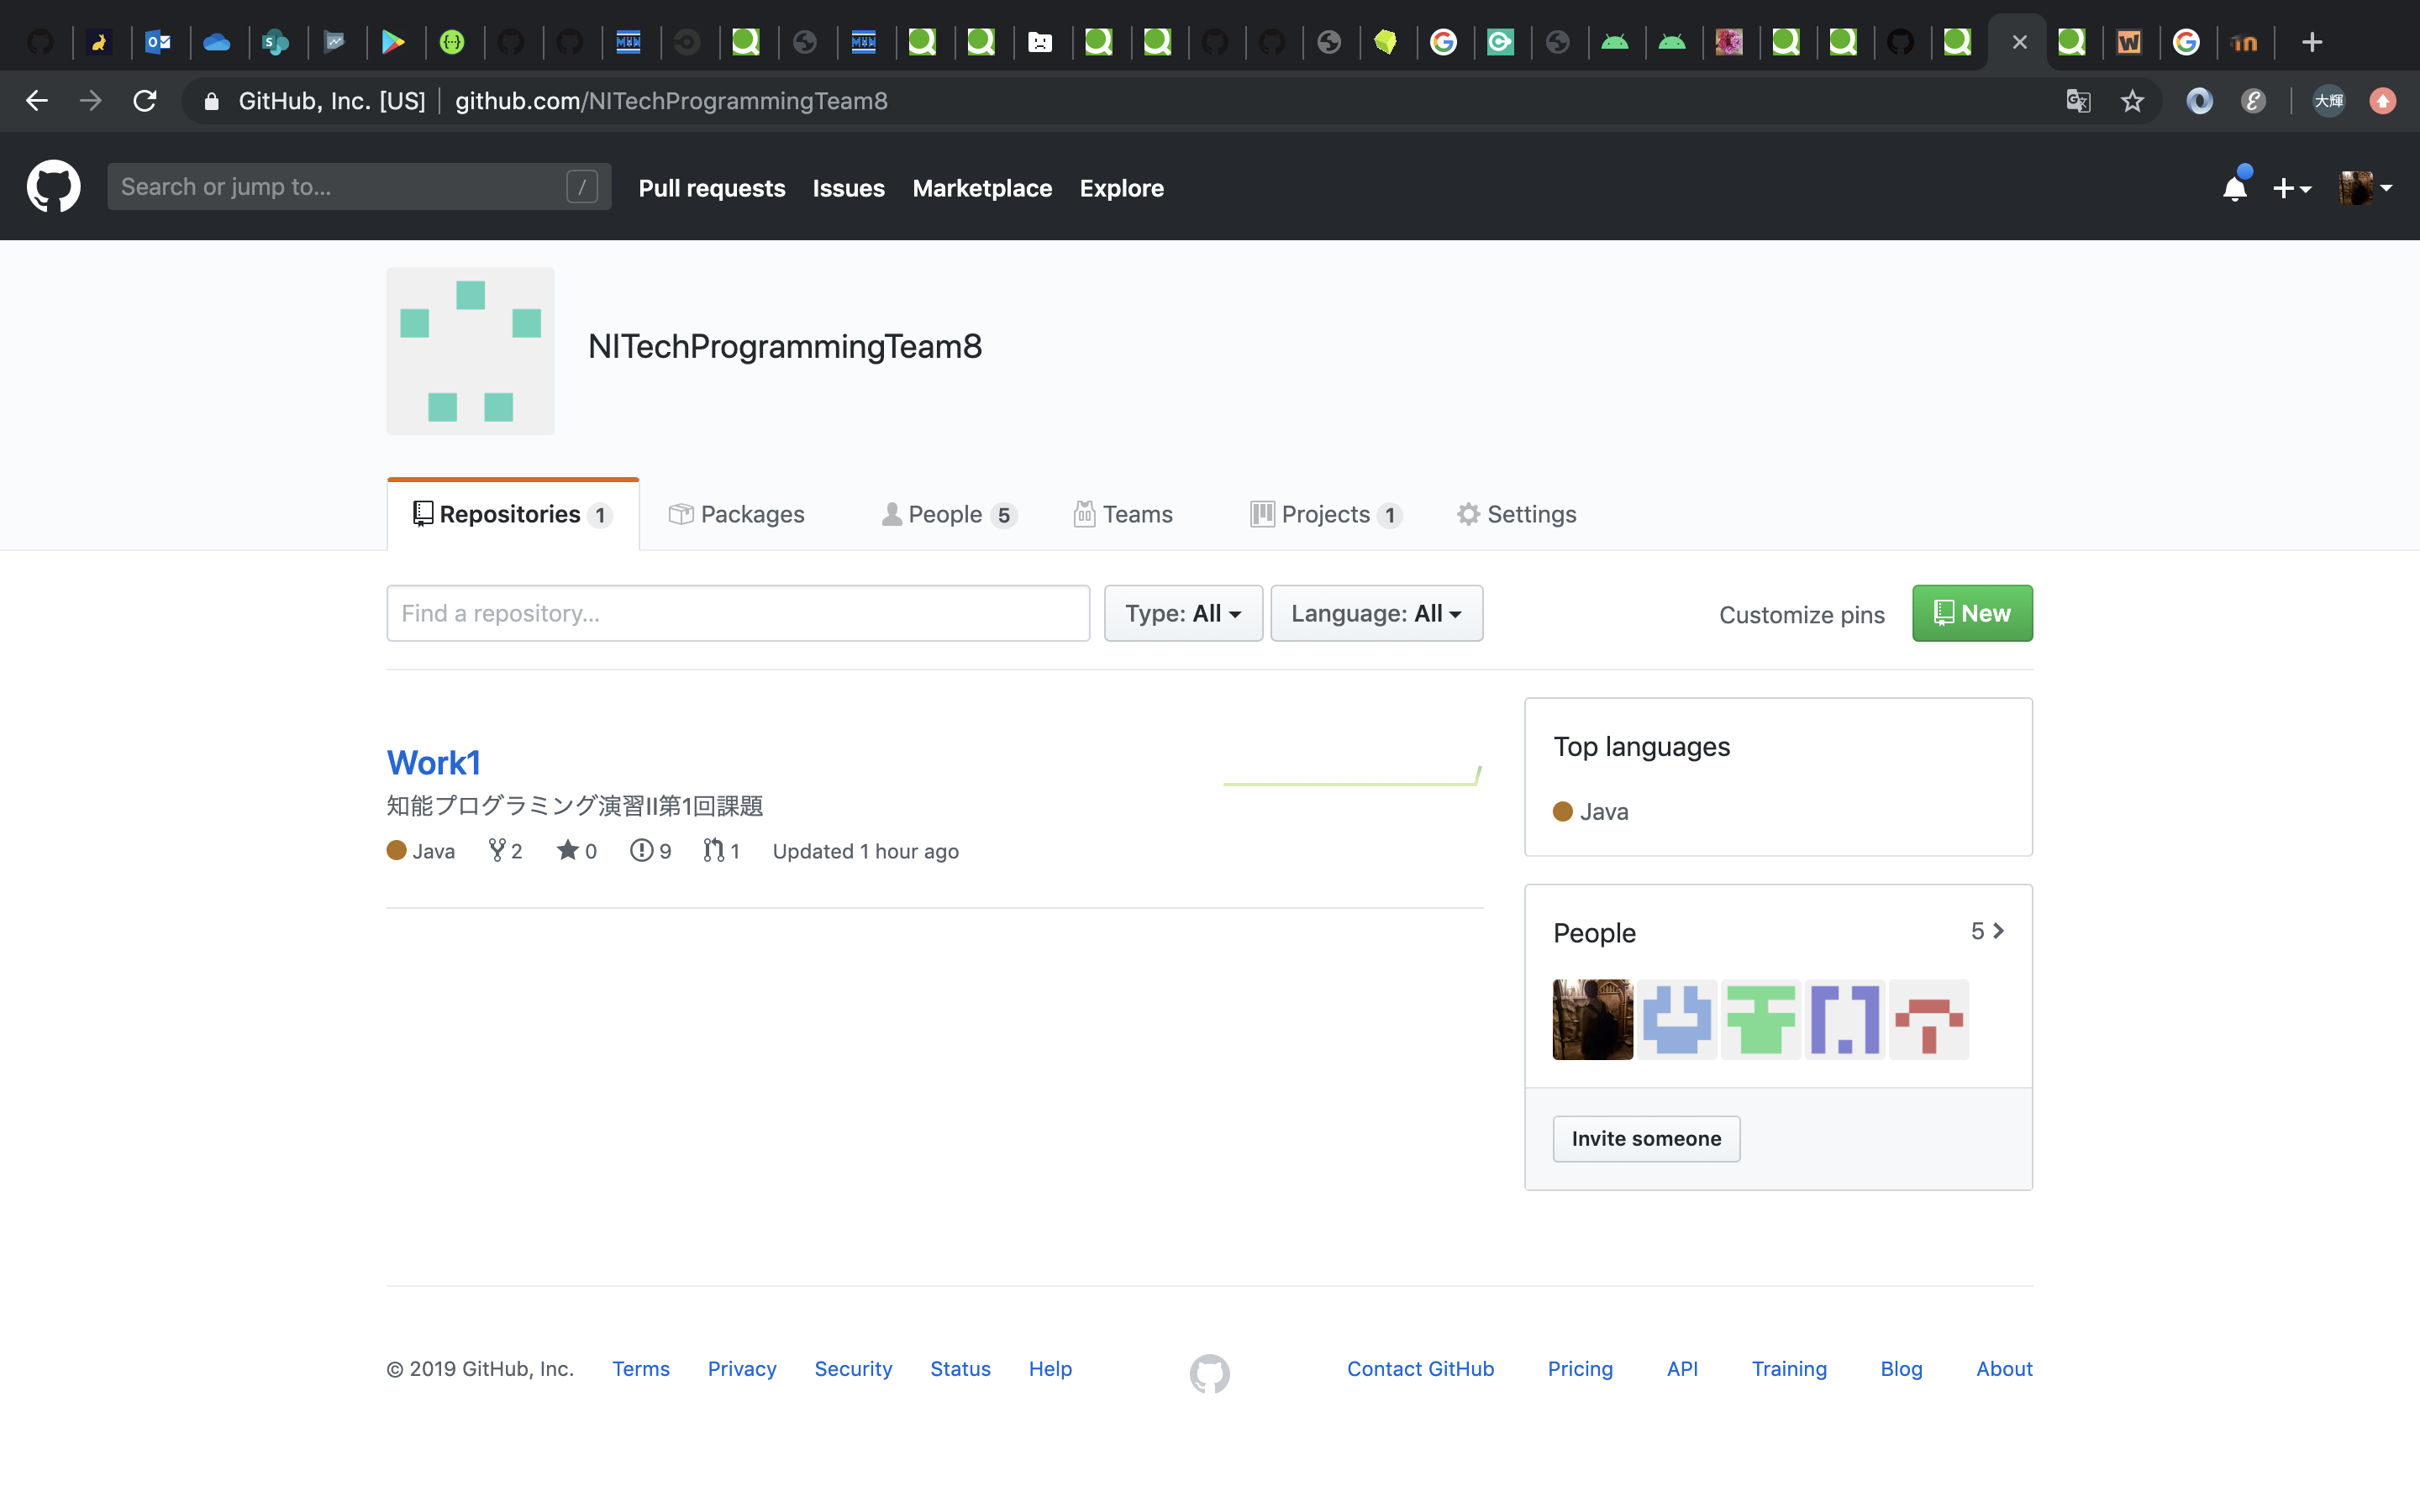
\includegraphics[scale=0.20]{git_image/organization_image.png}
  \caption{作成したOrganization}
\end{figure}

\newpage

\subsection{GitHubの導入}

次に,主に利用した機能を以下に列挙する. \\
\begin{description}
  \item[Project機能] Work1用のプロジェクトを作成し,進捗管理を行うためのカンバンとする.
  \item[Issues機能] 課題をいくつかのタスクに分解することにより,それぞれに担当者を割り当てる.
  \item[MileStones機能] 個々のIssuesを完了するまでの期間を定める.
  \item[PullRequest機能] 各Issuesと結びつけることによって,タスクと実際の作業を結びつける.
\end{description}

\subsection{Project機能の運用と考察}
今回はWork1というリポジトリに対応したProjectを作成した.
このProjectはカンバンと呼ばれ,プロジェクト全体の進行度を視覚的に把握するのに最適である. \\
今回はタスクの進行度を以下の3種類に分類し,Columnに登録した. \\
さらに,PRへの割当やMergeといったイベントを完了することによって,タスクの進行度が変化するように自動化を行った.
\begin{description}
  \item[To do] これから着手する予定のタスク.PR発行時にDevelopingに移動する.
  \item[Developing] 開発中のタスク.Merge後にDoneに移動する.
  \item[Done] 完了後のタスク.
\end{description}
発行したIssuesをタスクとすることでカンバンにおけるカードとした.
以下に,Projectの画像を添付する.

\begin{figure}[!hbt]
  \centering
  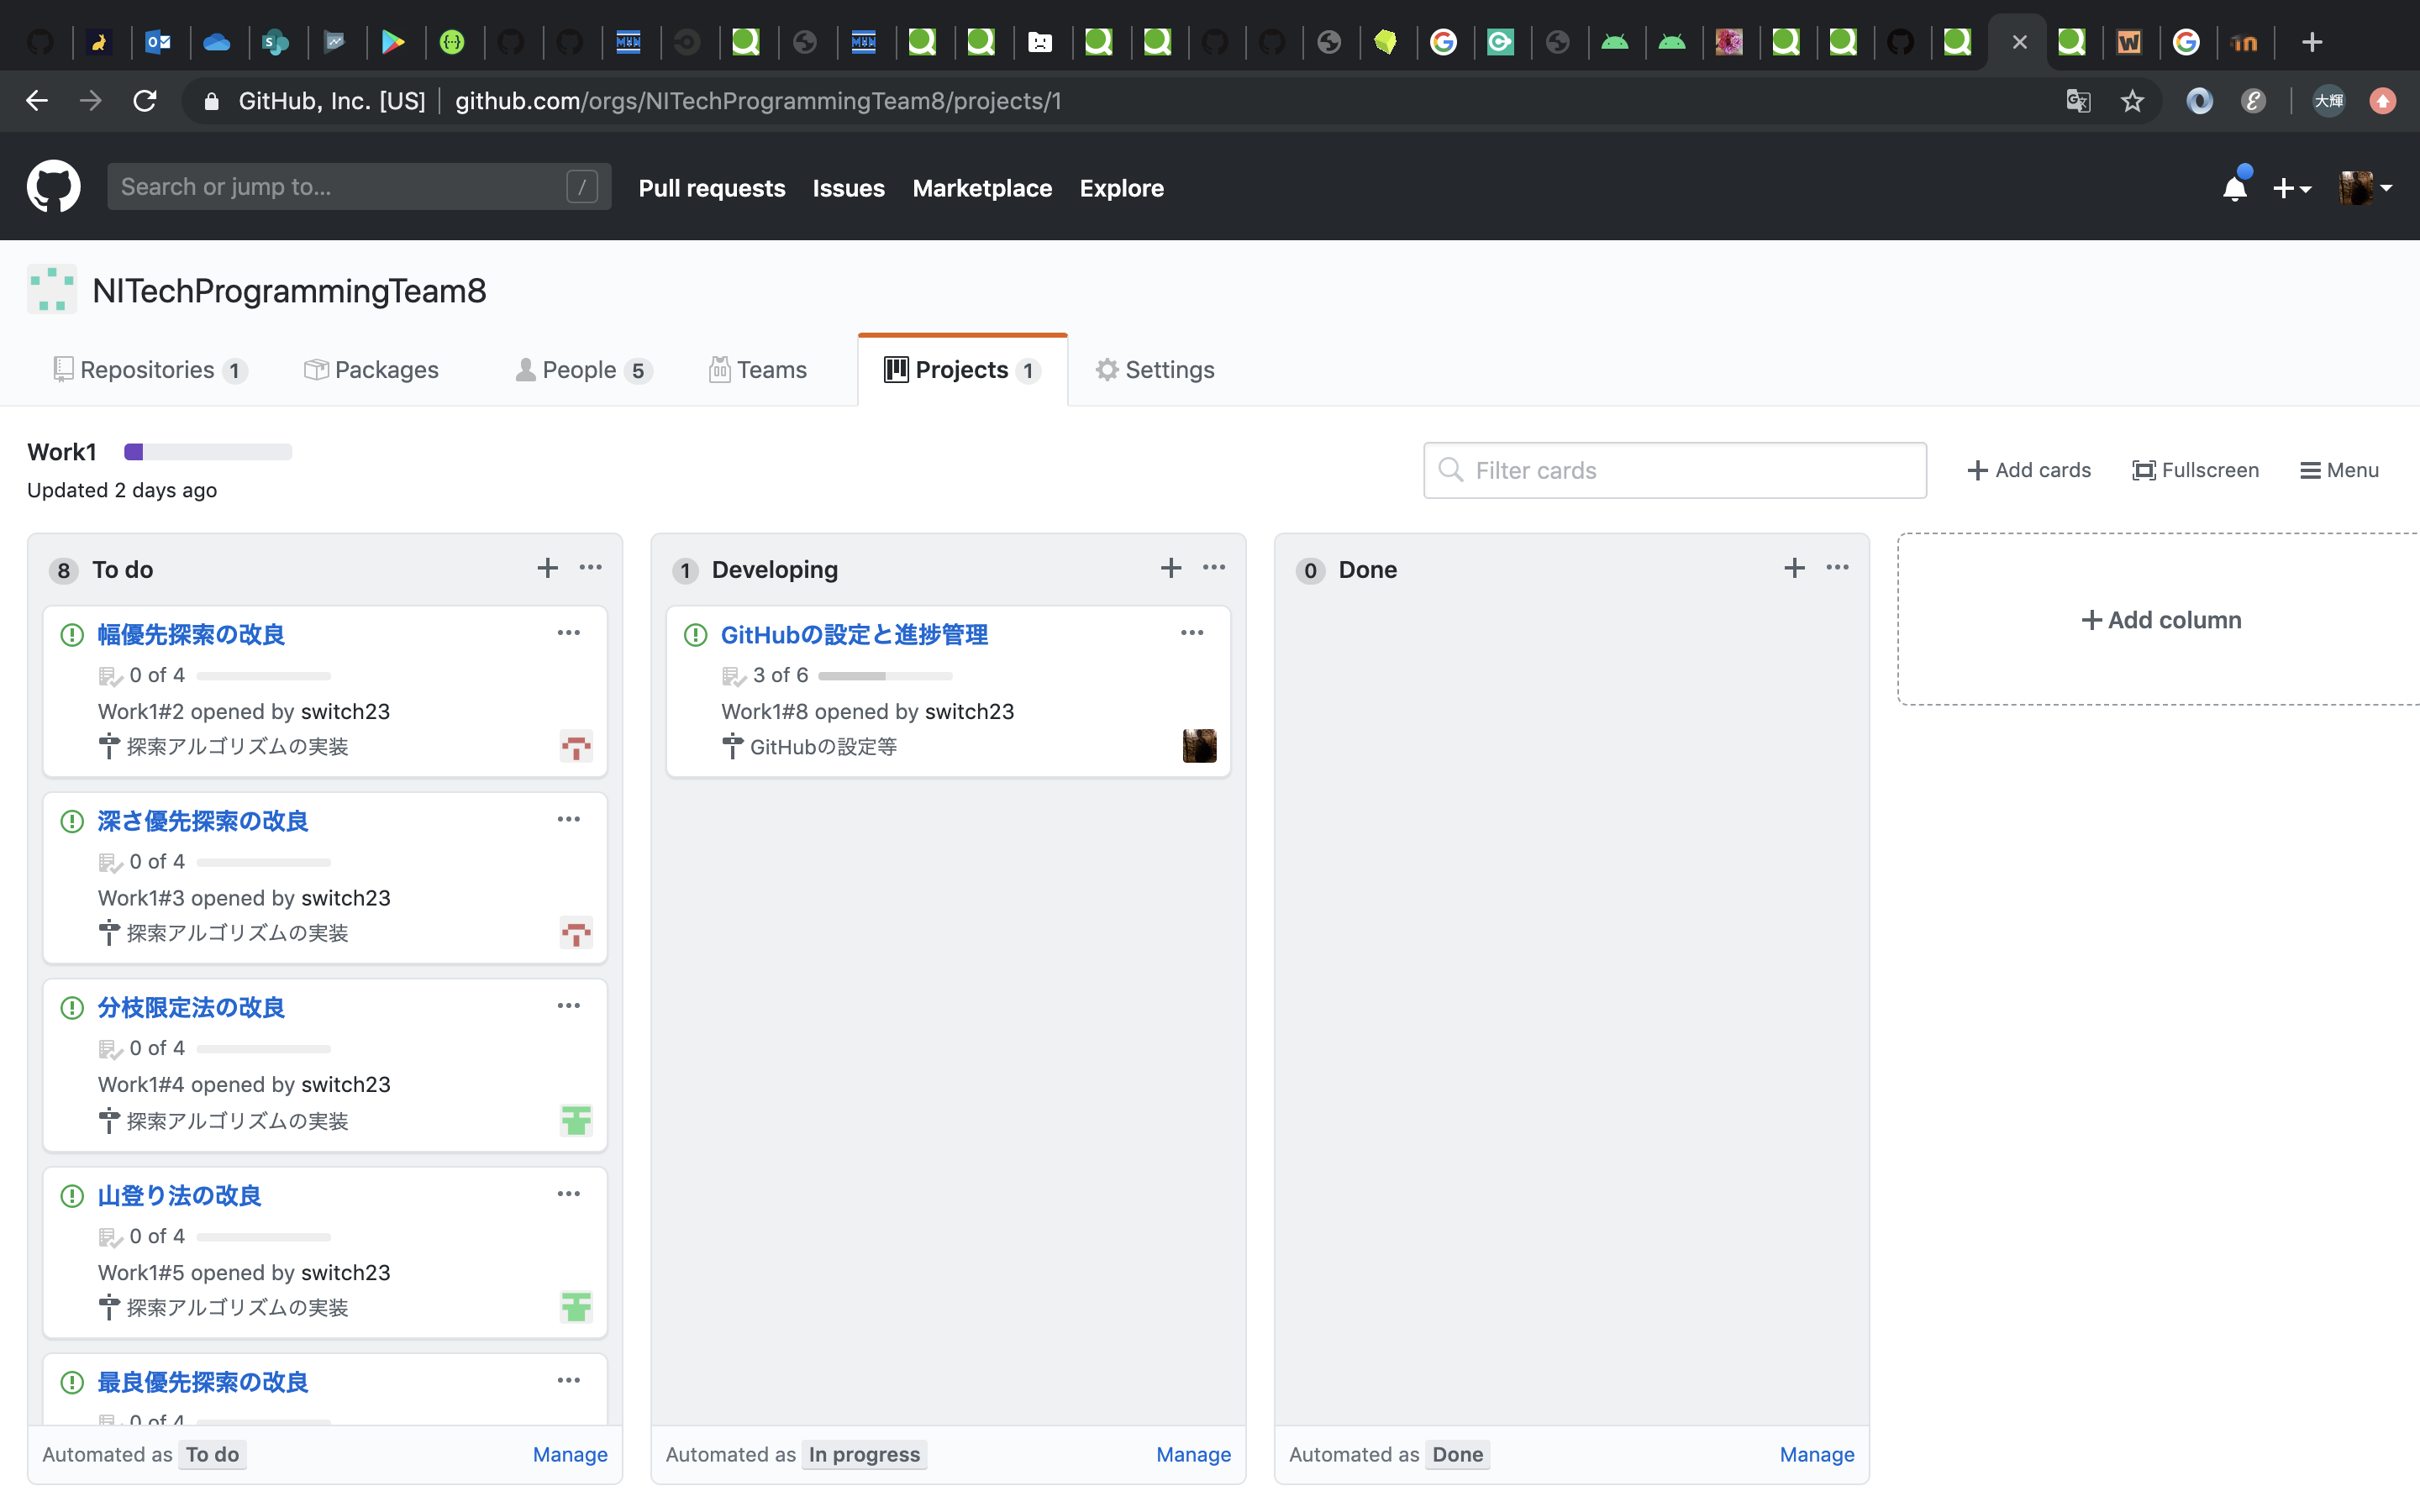
\includegraphics[scale=0.25]{git_image/project_image.png}
  \caption{Project機能を用いたタスク管理}
\end{figure}

\newpage


\subsection{Issues機能の運用と考察}
今回はタスクに対応したIssuesを発行した.
それぞれのIssuesには最低1人の担当者を割り当て,MileStones機能により期日を設けた. \\
次のようにタスクを分解し,Issuesを発行した.
\begin{description}
  \item[幅優先探索]
  \item[深さ優先探索]
  \item[最良優先探索]
  \item[A*アルゴリズム]
  \item[分枝限定法]
  \item[山登り法]
  \item[GitHub管理]
  \item[GUI設計]     
\end{description}
また,個々のタスクはさらに粒度の細かい作業に分解され,それぞれに対してチェック欄を設け,メンバー全体が各々の進捗状況を細かく確認できる仕様にした.
以下に,Issuesの画像を添付する.

\begin{figure}[!hbt]
  \centering
  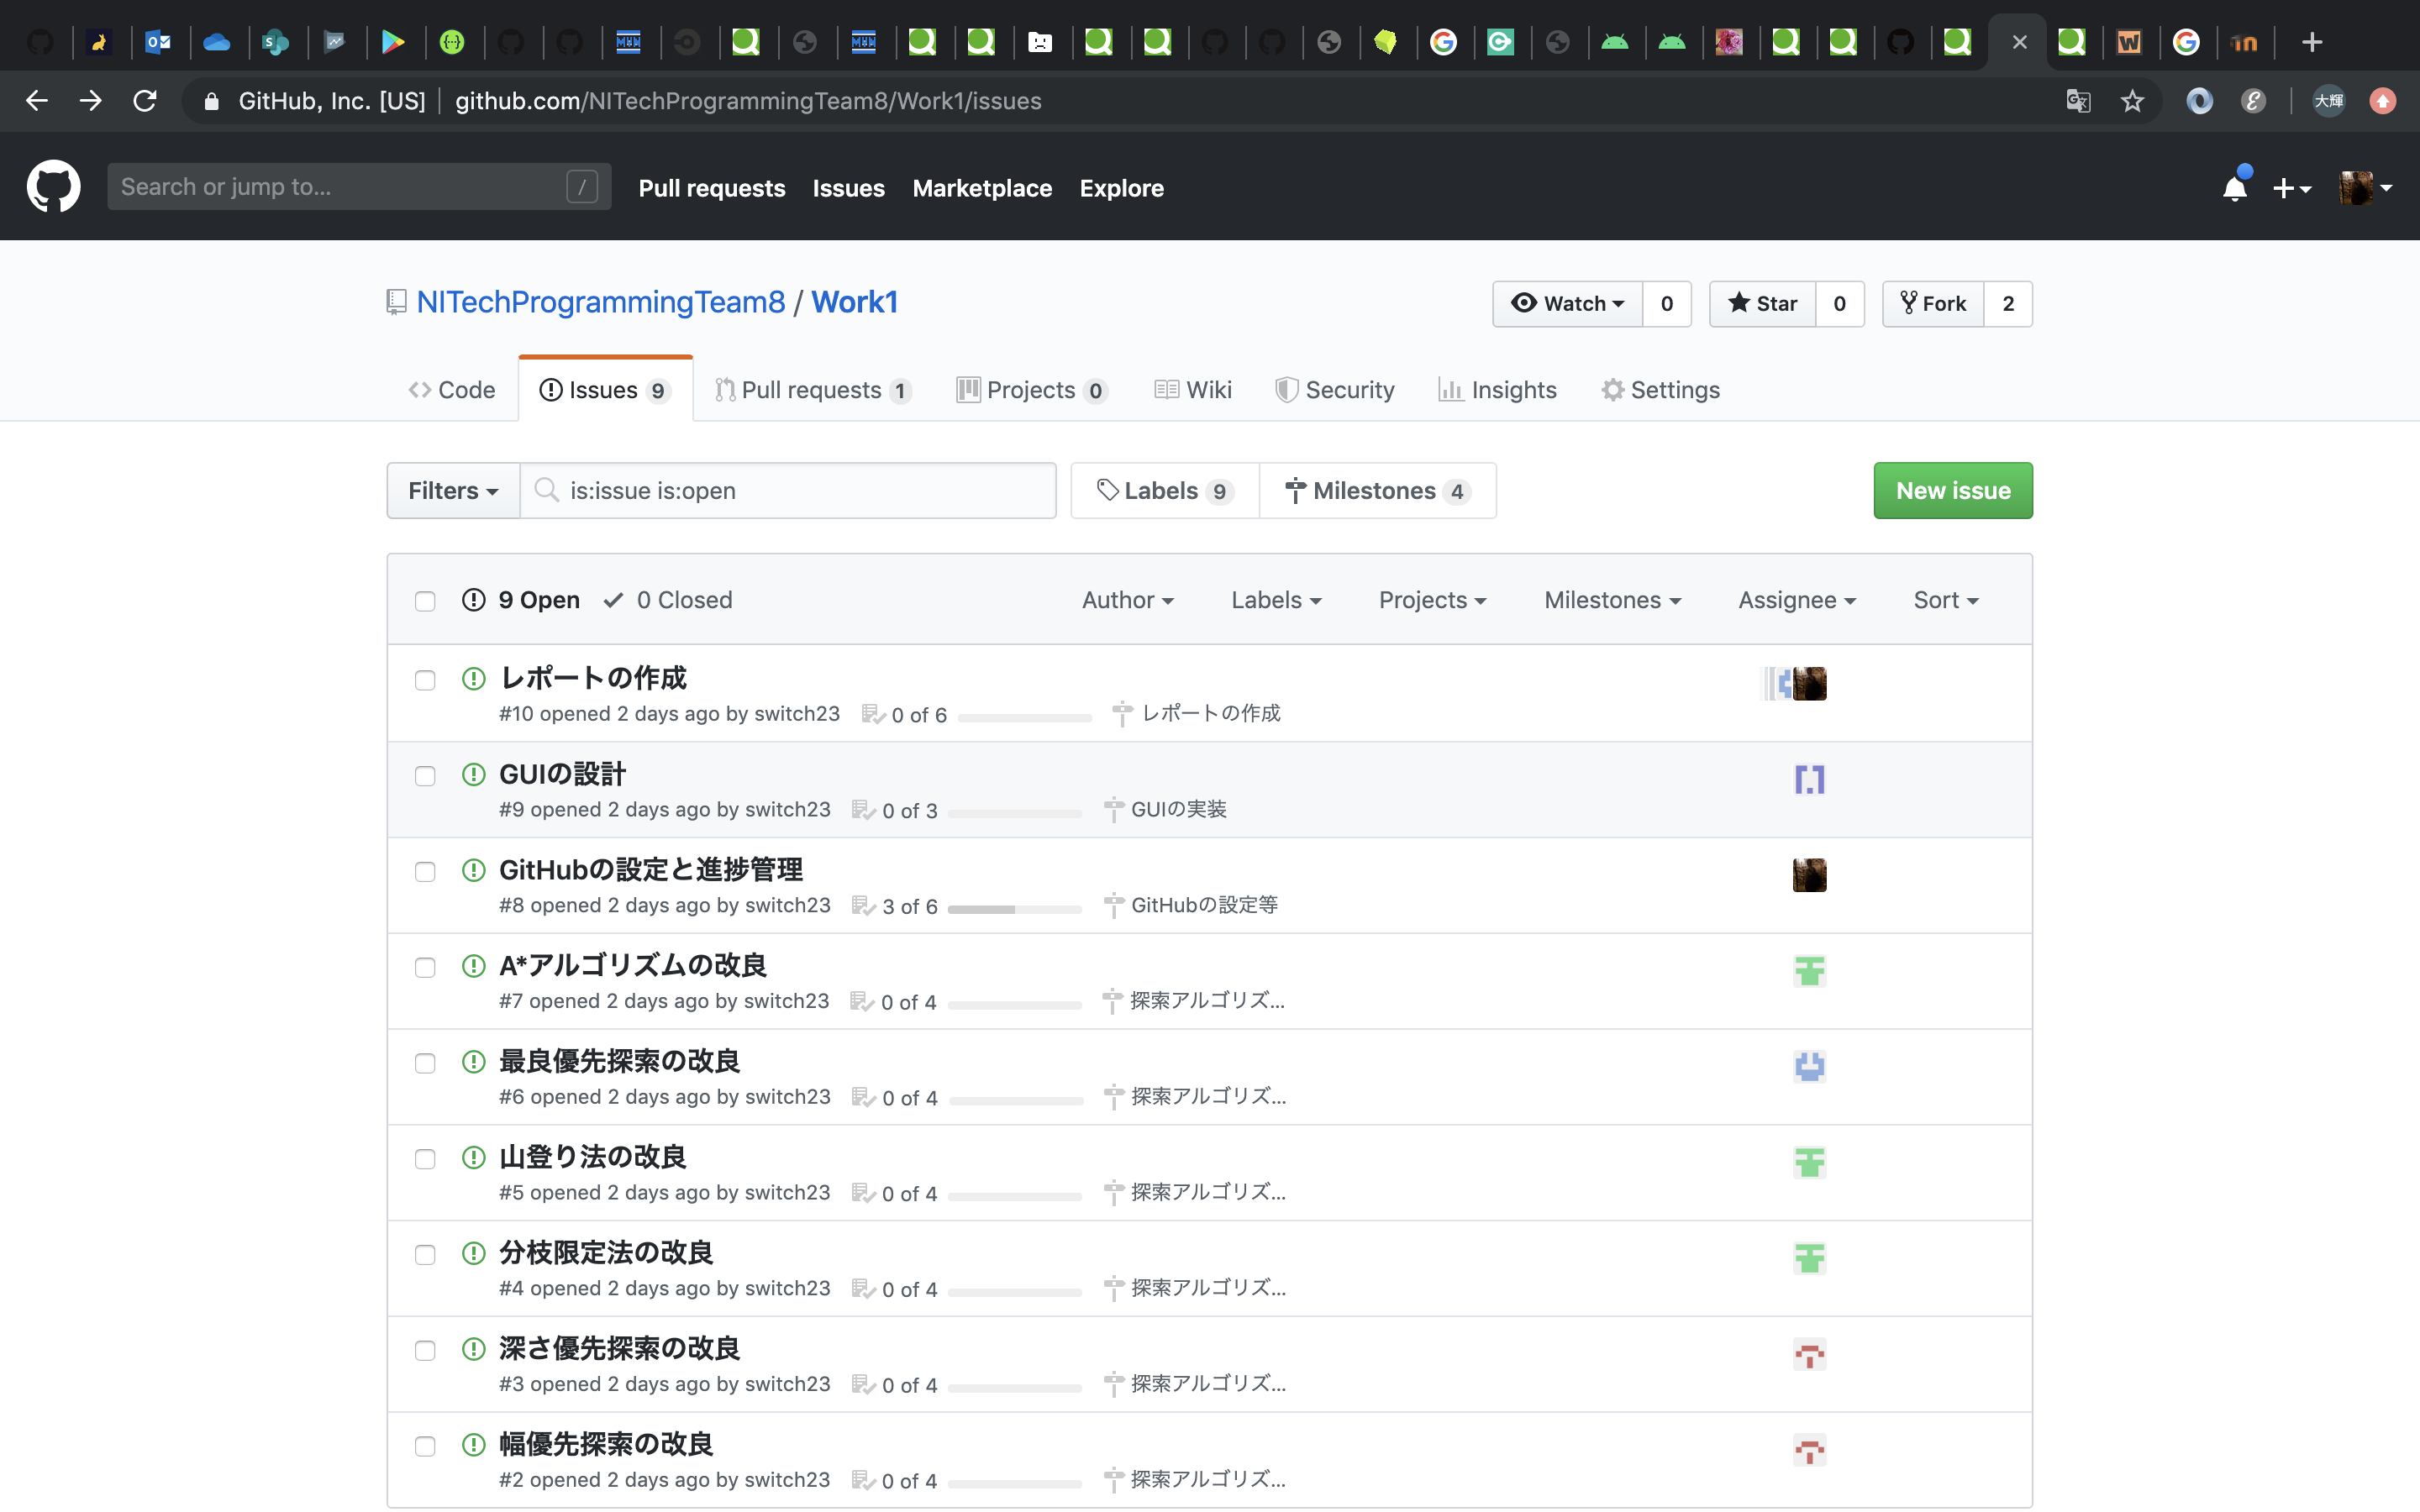
\includegraphics[scale=0.20]{git_image/issues_list_image.png}
  \caption{Issues一覧}
\end{figure}

\begin{figure}[!hbt]
  \centering
  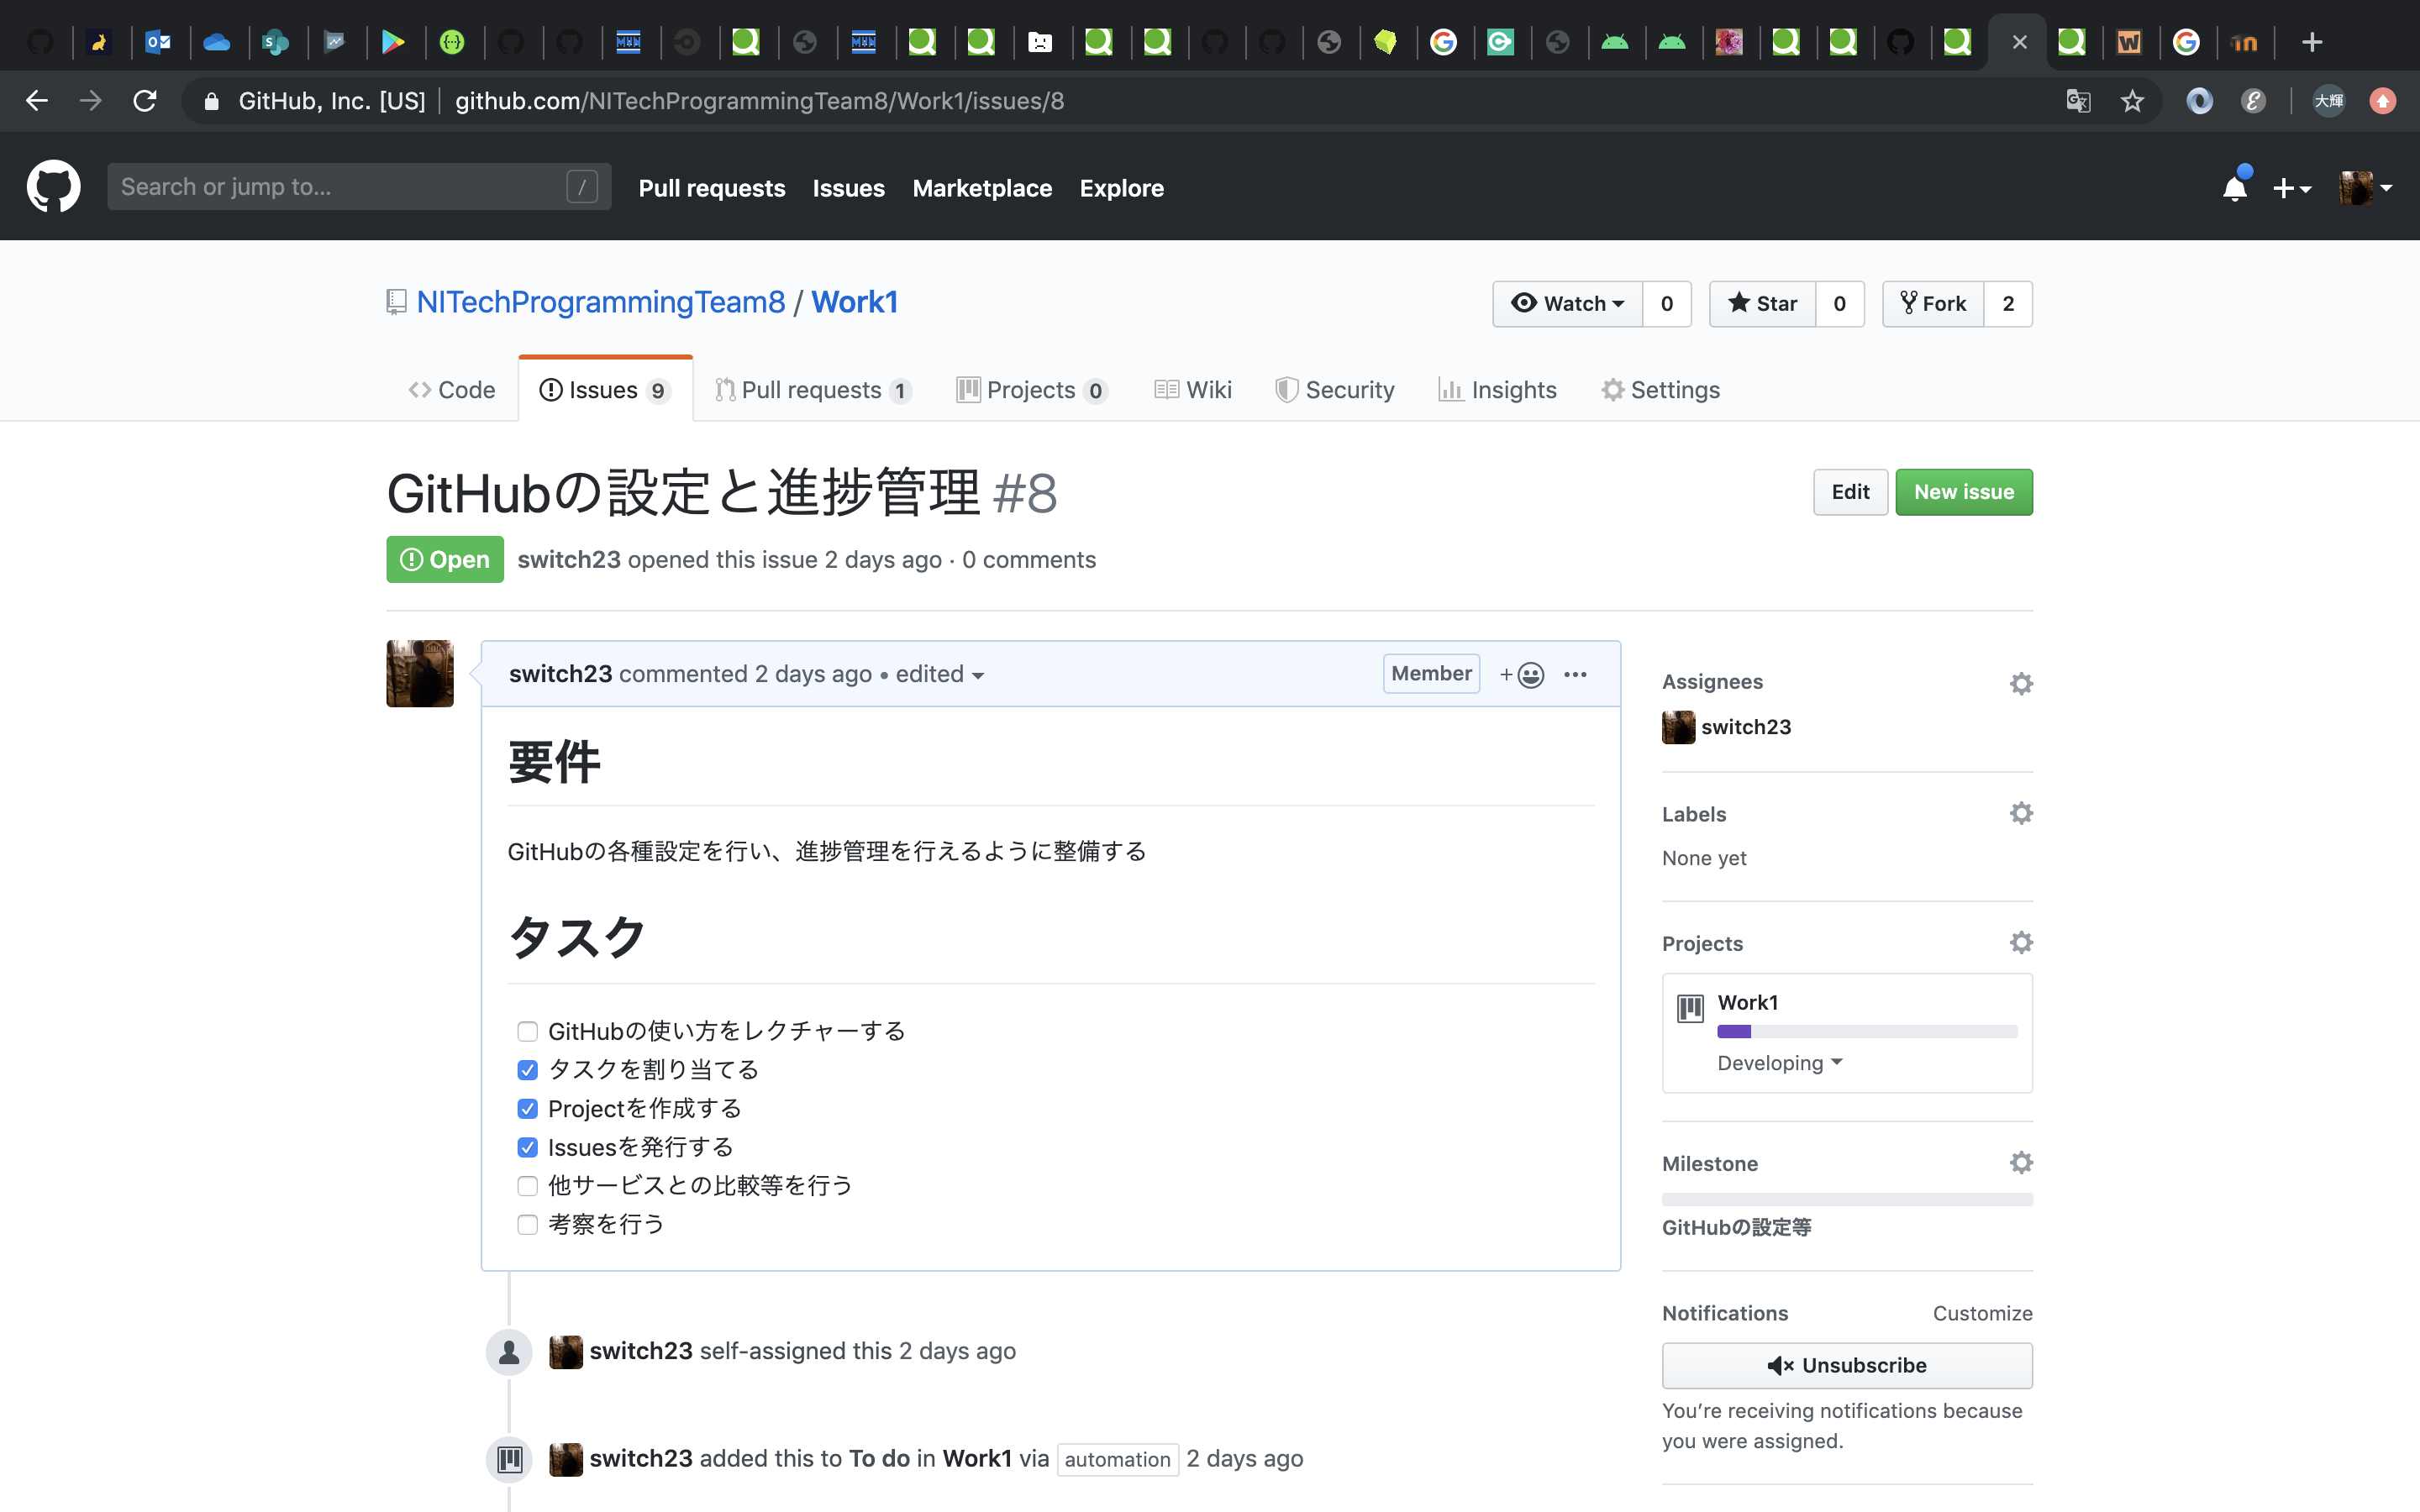
\includegraphics[scale=0.20]{git_image/issues_image.png}
  \caption{Issues機能を用いたタスク割り当てとタスク分解}
\end{figure}

\newpage


\subsection{MileStones機能の運用と考察}
今回は個々のタスクを終了すべき期日をMileStones機能により設定した.
設定したMileStonesは以下の通りである. \\
\begin{description}
  \item[探索アルゴリズムの実装] 10/10(木)
  \item[GitHubの設定等] 10/10(木)
  \item[GUIの実装] 10/13(日)
  \item[レポートの作成] 10/13(日)
\end{description}

\begin{figure}[!hbt]
  \centering
  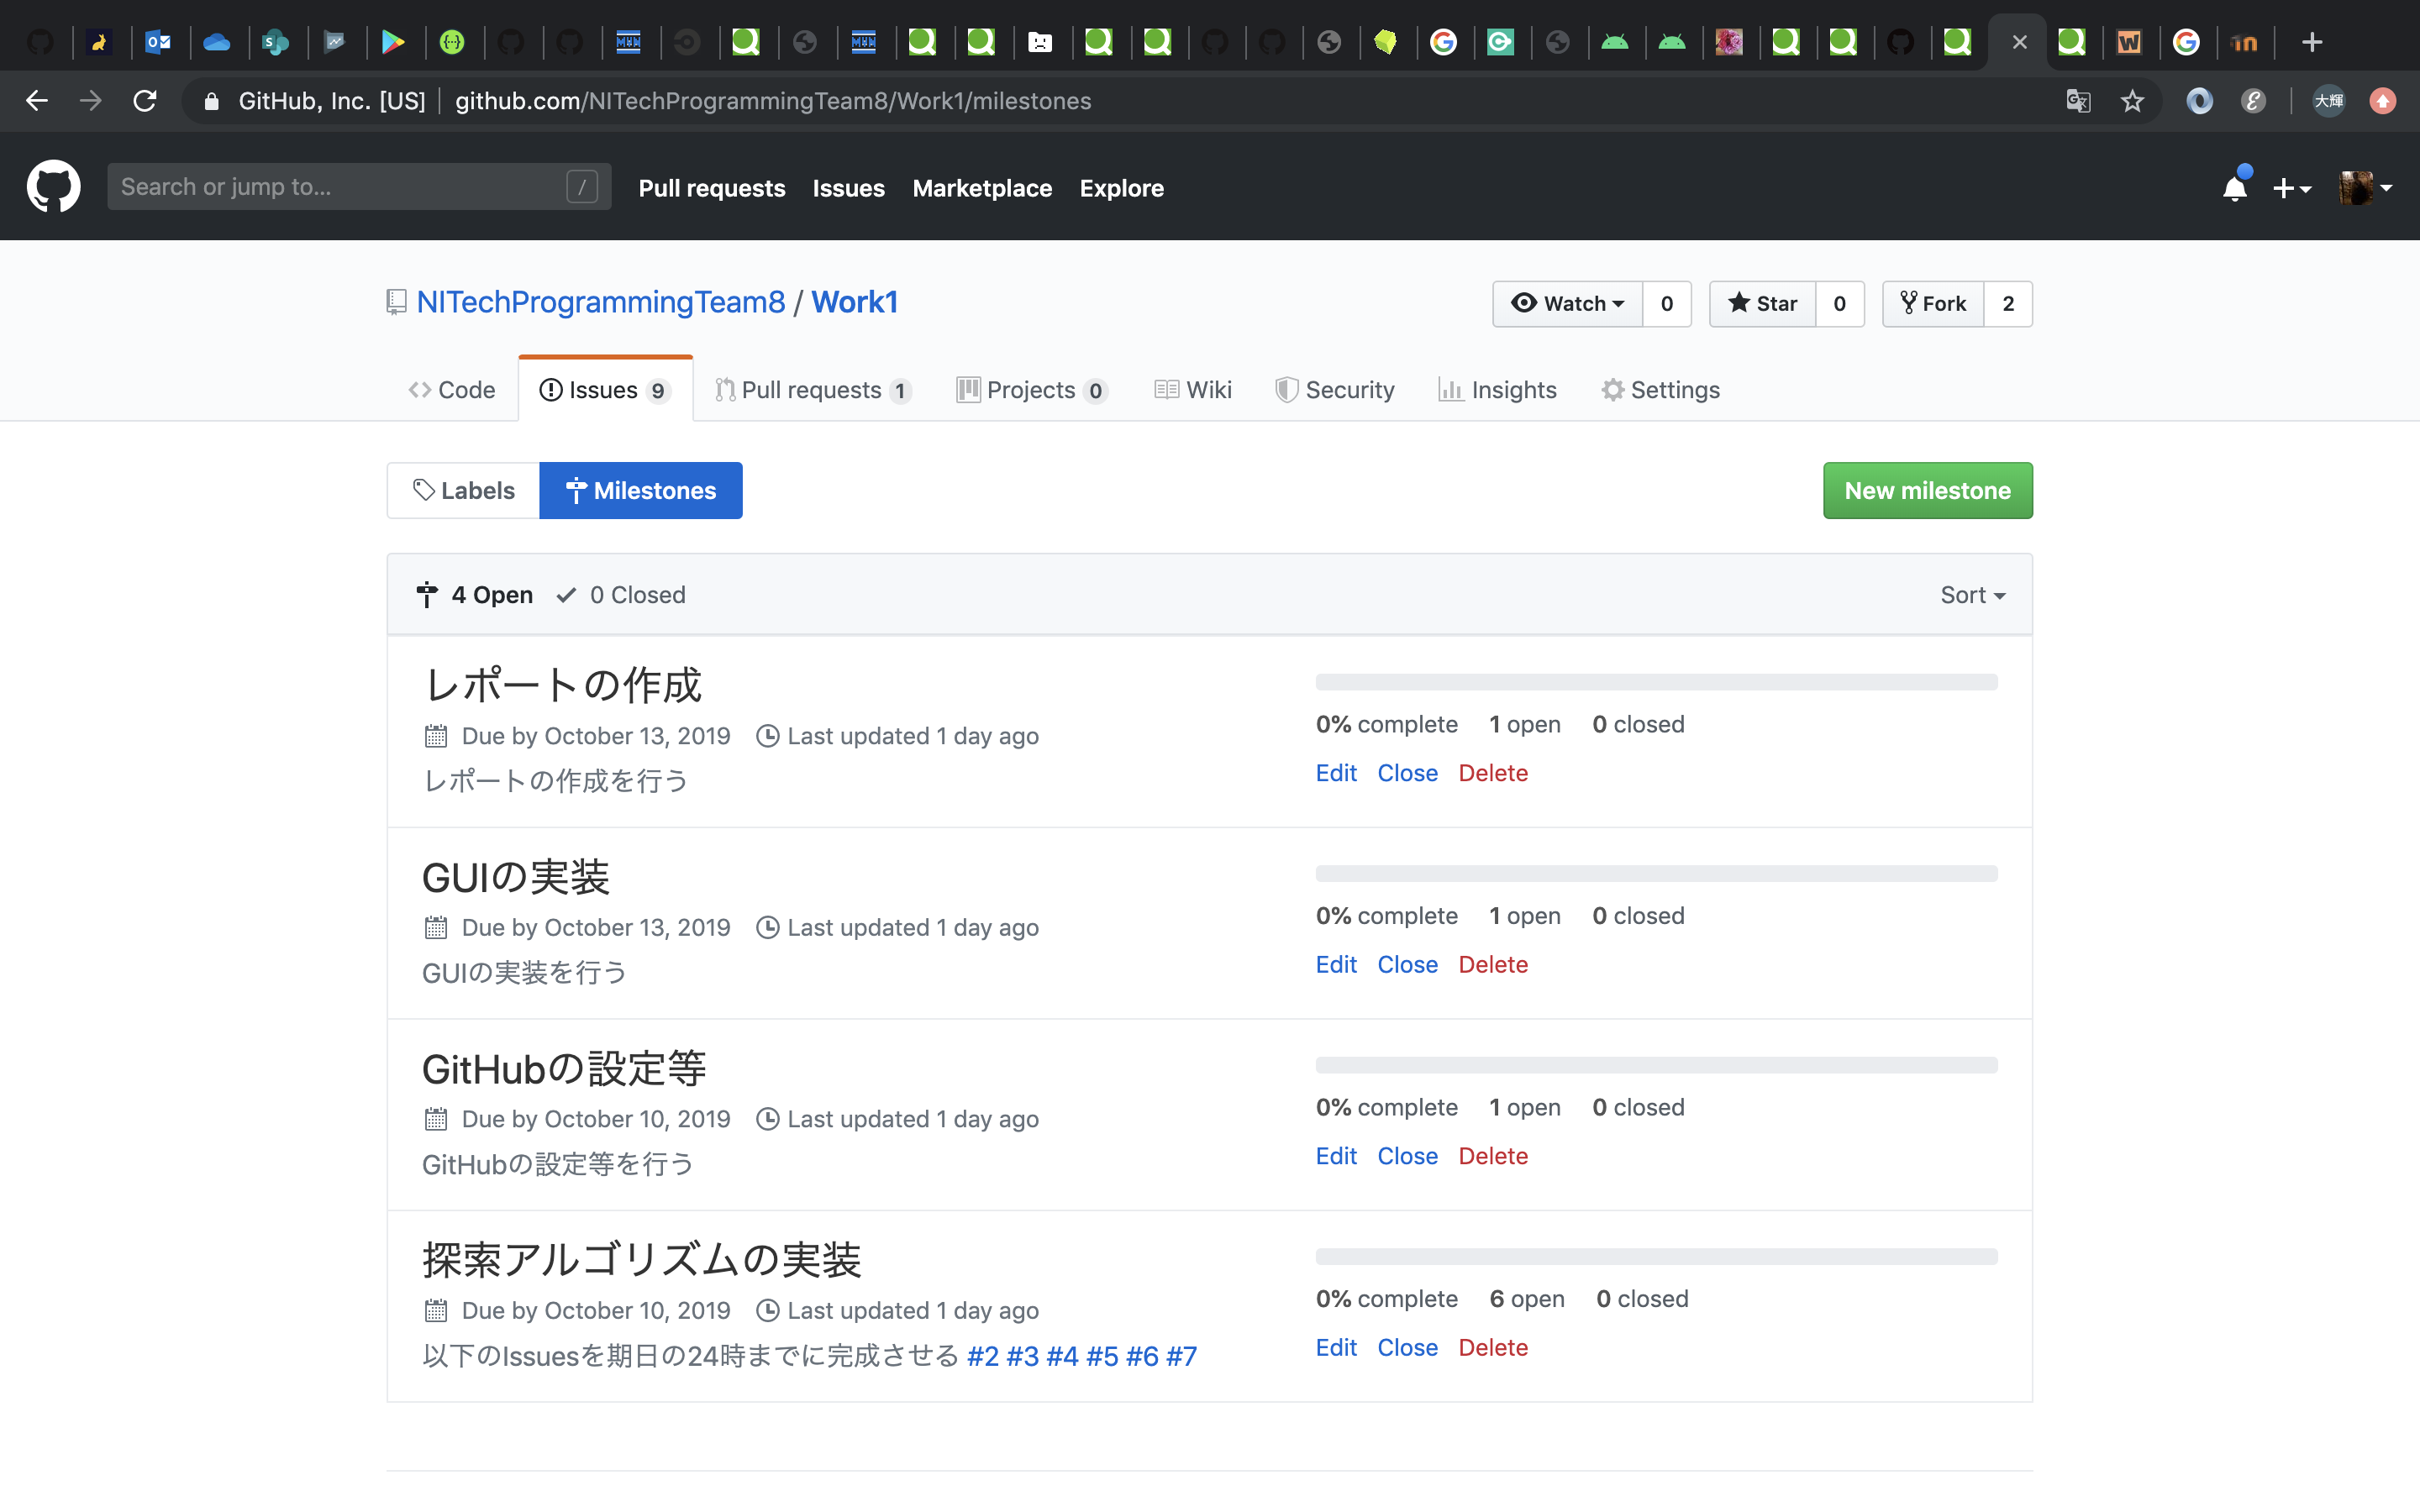
\includegraphics[scale=0.20]{git_image/milestones_list_image.png}
  \caption{MileStones一覧}
\end{figure}

\begin{figure}[!hbt]
  \centering
  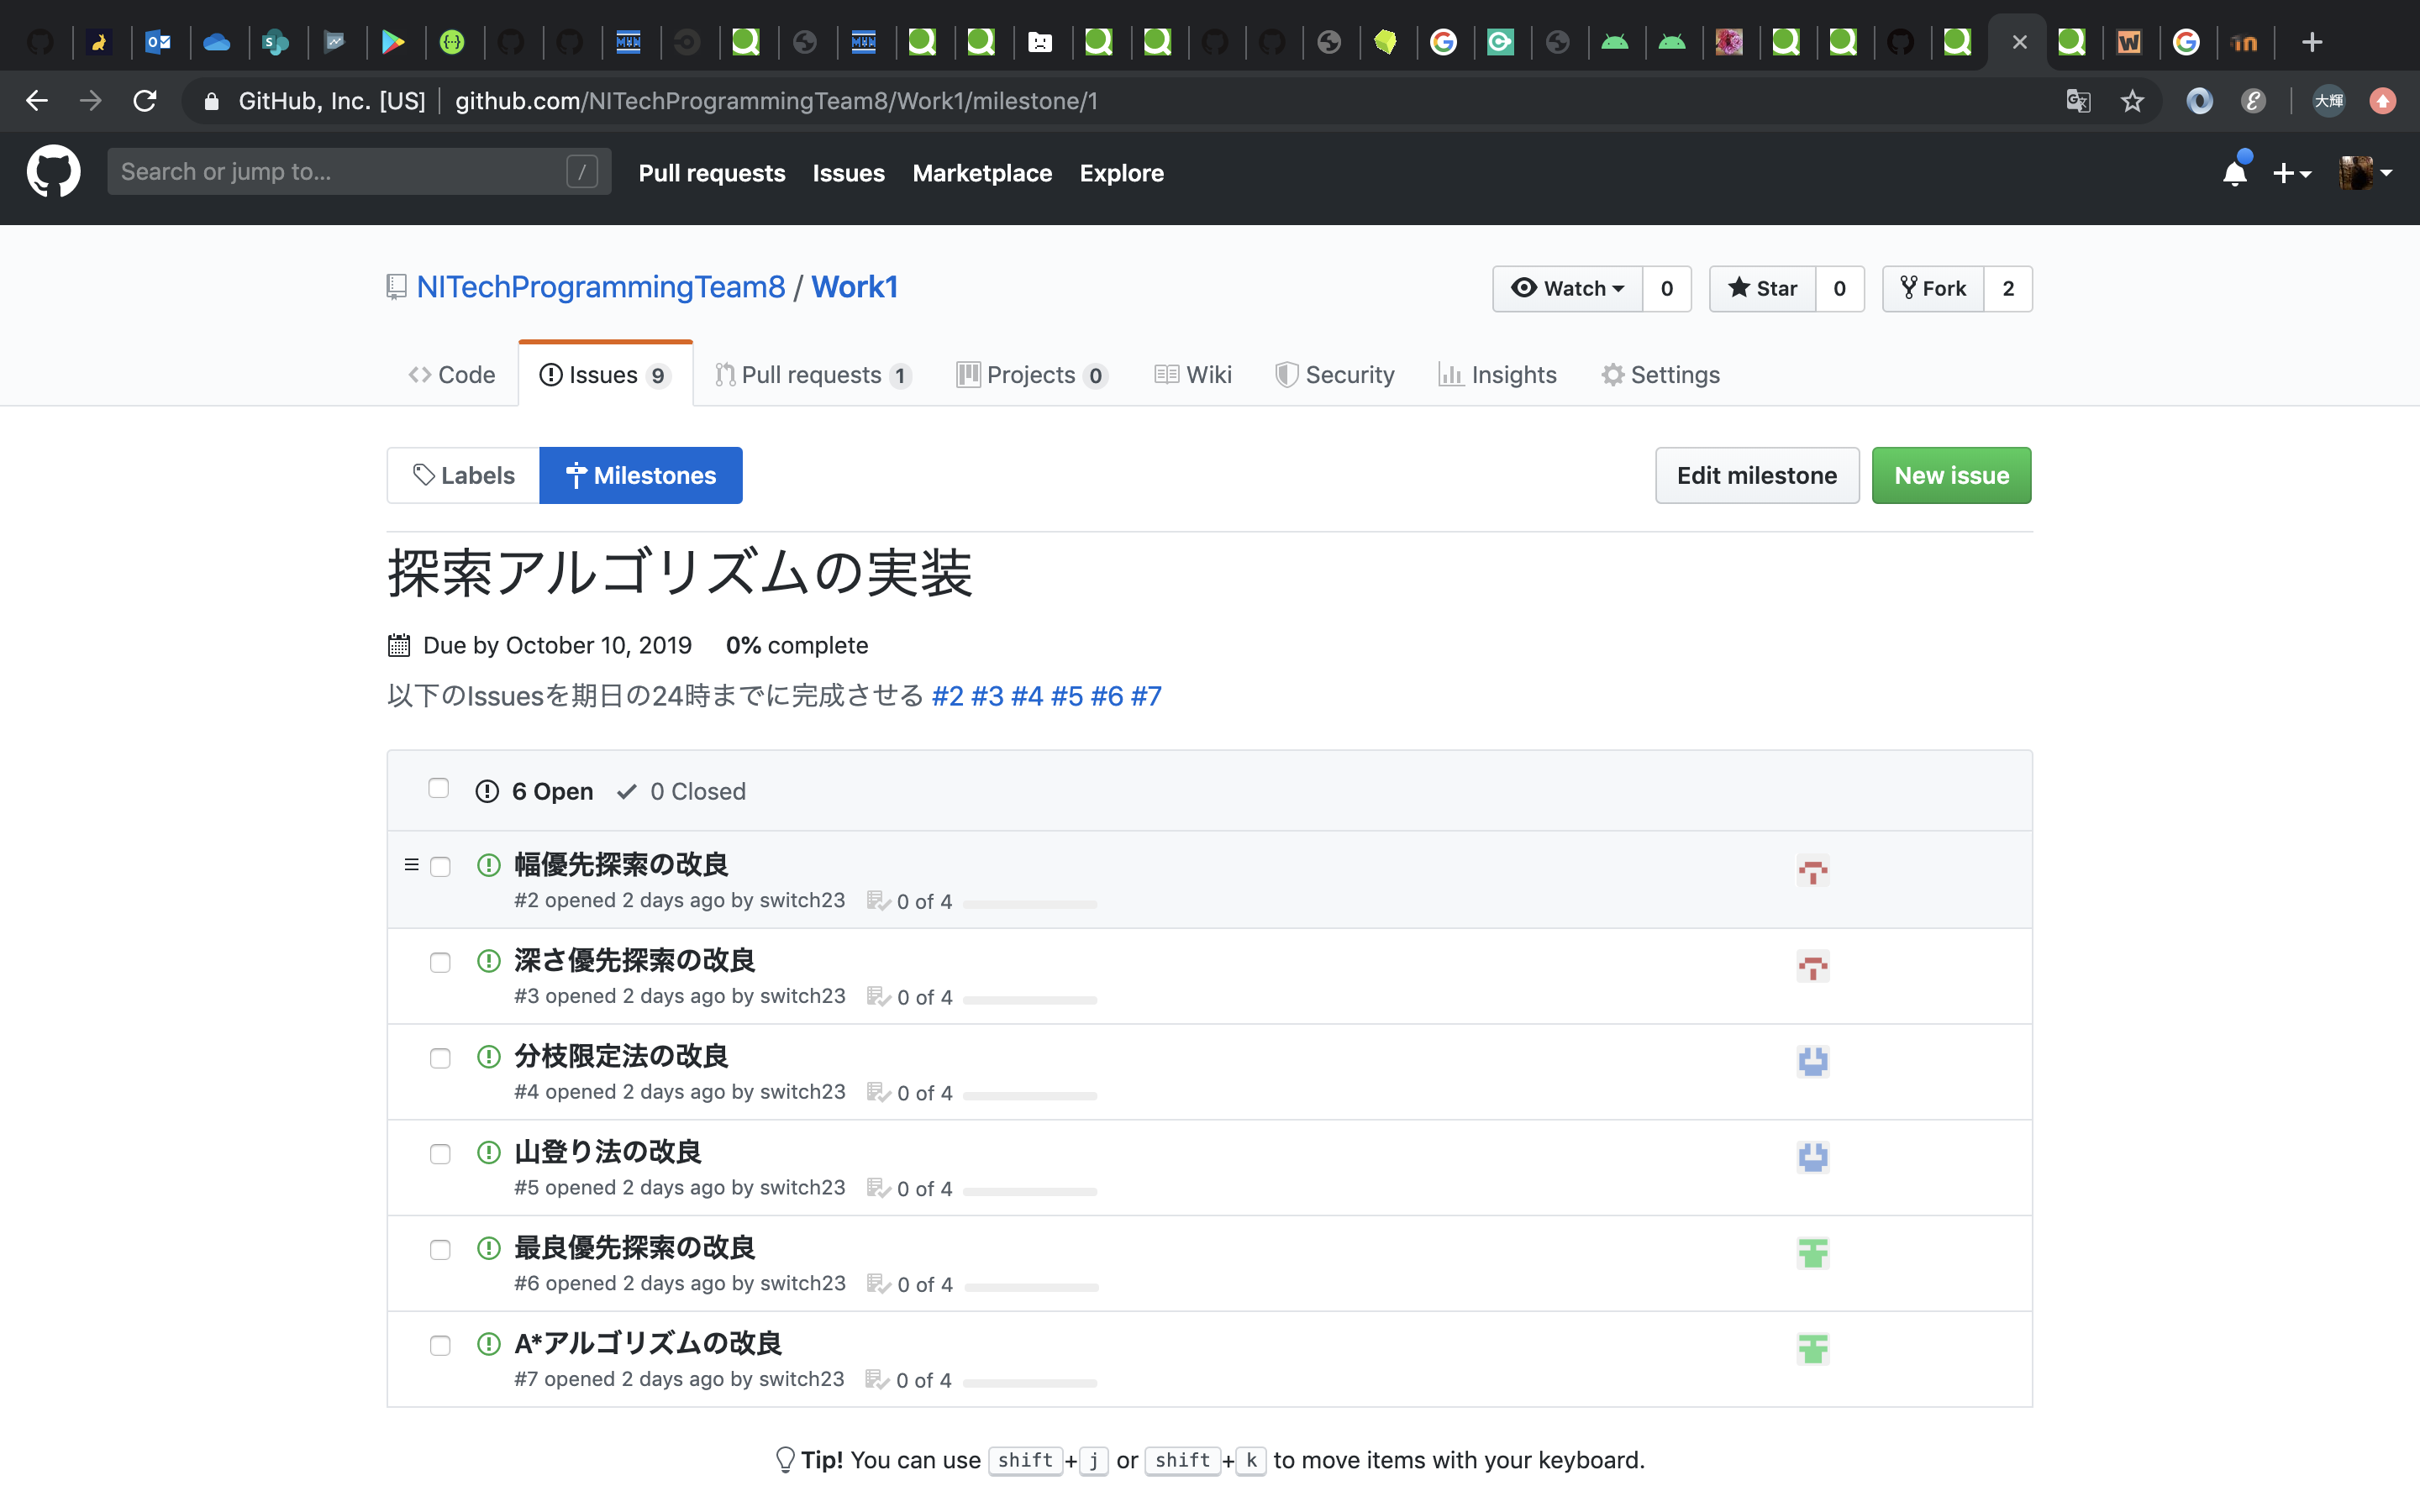
\includegraphics[scale=0.20]{git_image/milestones_image.png}
  \caption{MileStones機能を用いたIssuesの期日管理}
\end{figure}

\newpage


\subsection{PullRequest機能の運用と考察}
今回はIssues単位でPRを発行し,紐づけるものとする. \\
PRを行うことによって,変更をmasterブランチにMergeする前にレビューを行い,事前に問題点などを吟味することができる. \\
また,masterとの差分によって変更点を視覚的に示すことが可能なため,メンバーの詳細な作業内容を把握しやすく,ソースコードの共有が容易となる. \\
さらに,何か議論がある場合には,PR上で当該コードを指定してコメントを残すことができるため,具体性が増すメリットがある. \\
以上のようにPR機能を用いることによって,ソースコードの品質を維持するだけでなく,円滑なコミュニティを形成することが可能となる.

\begin{figure}[!hbt]
  \centering
  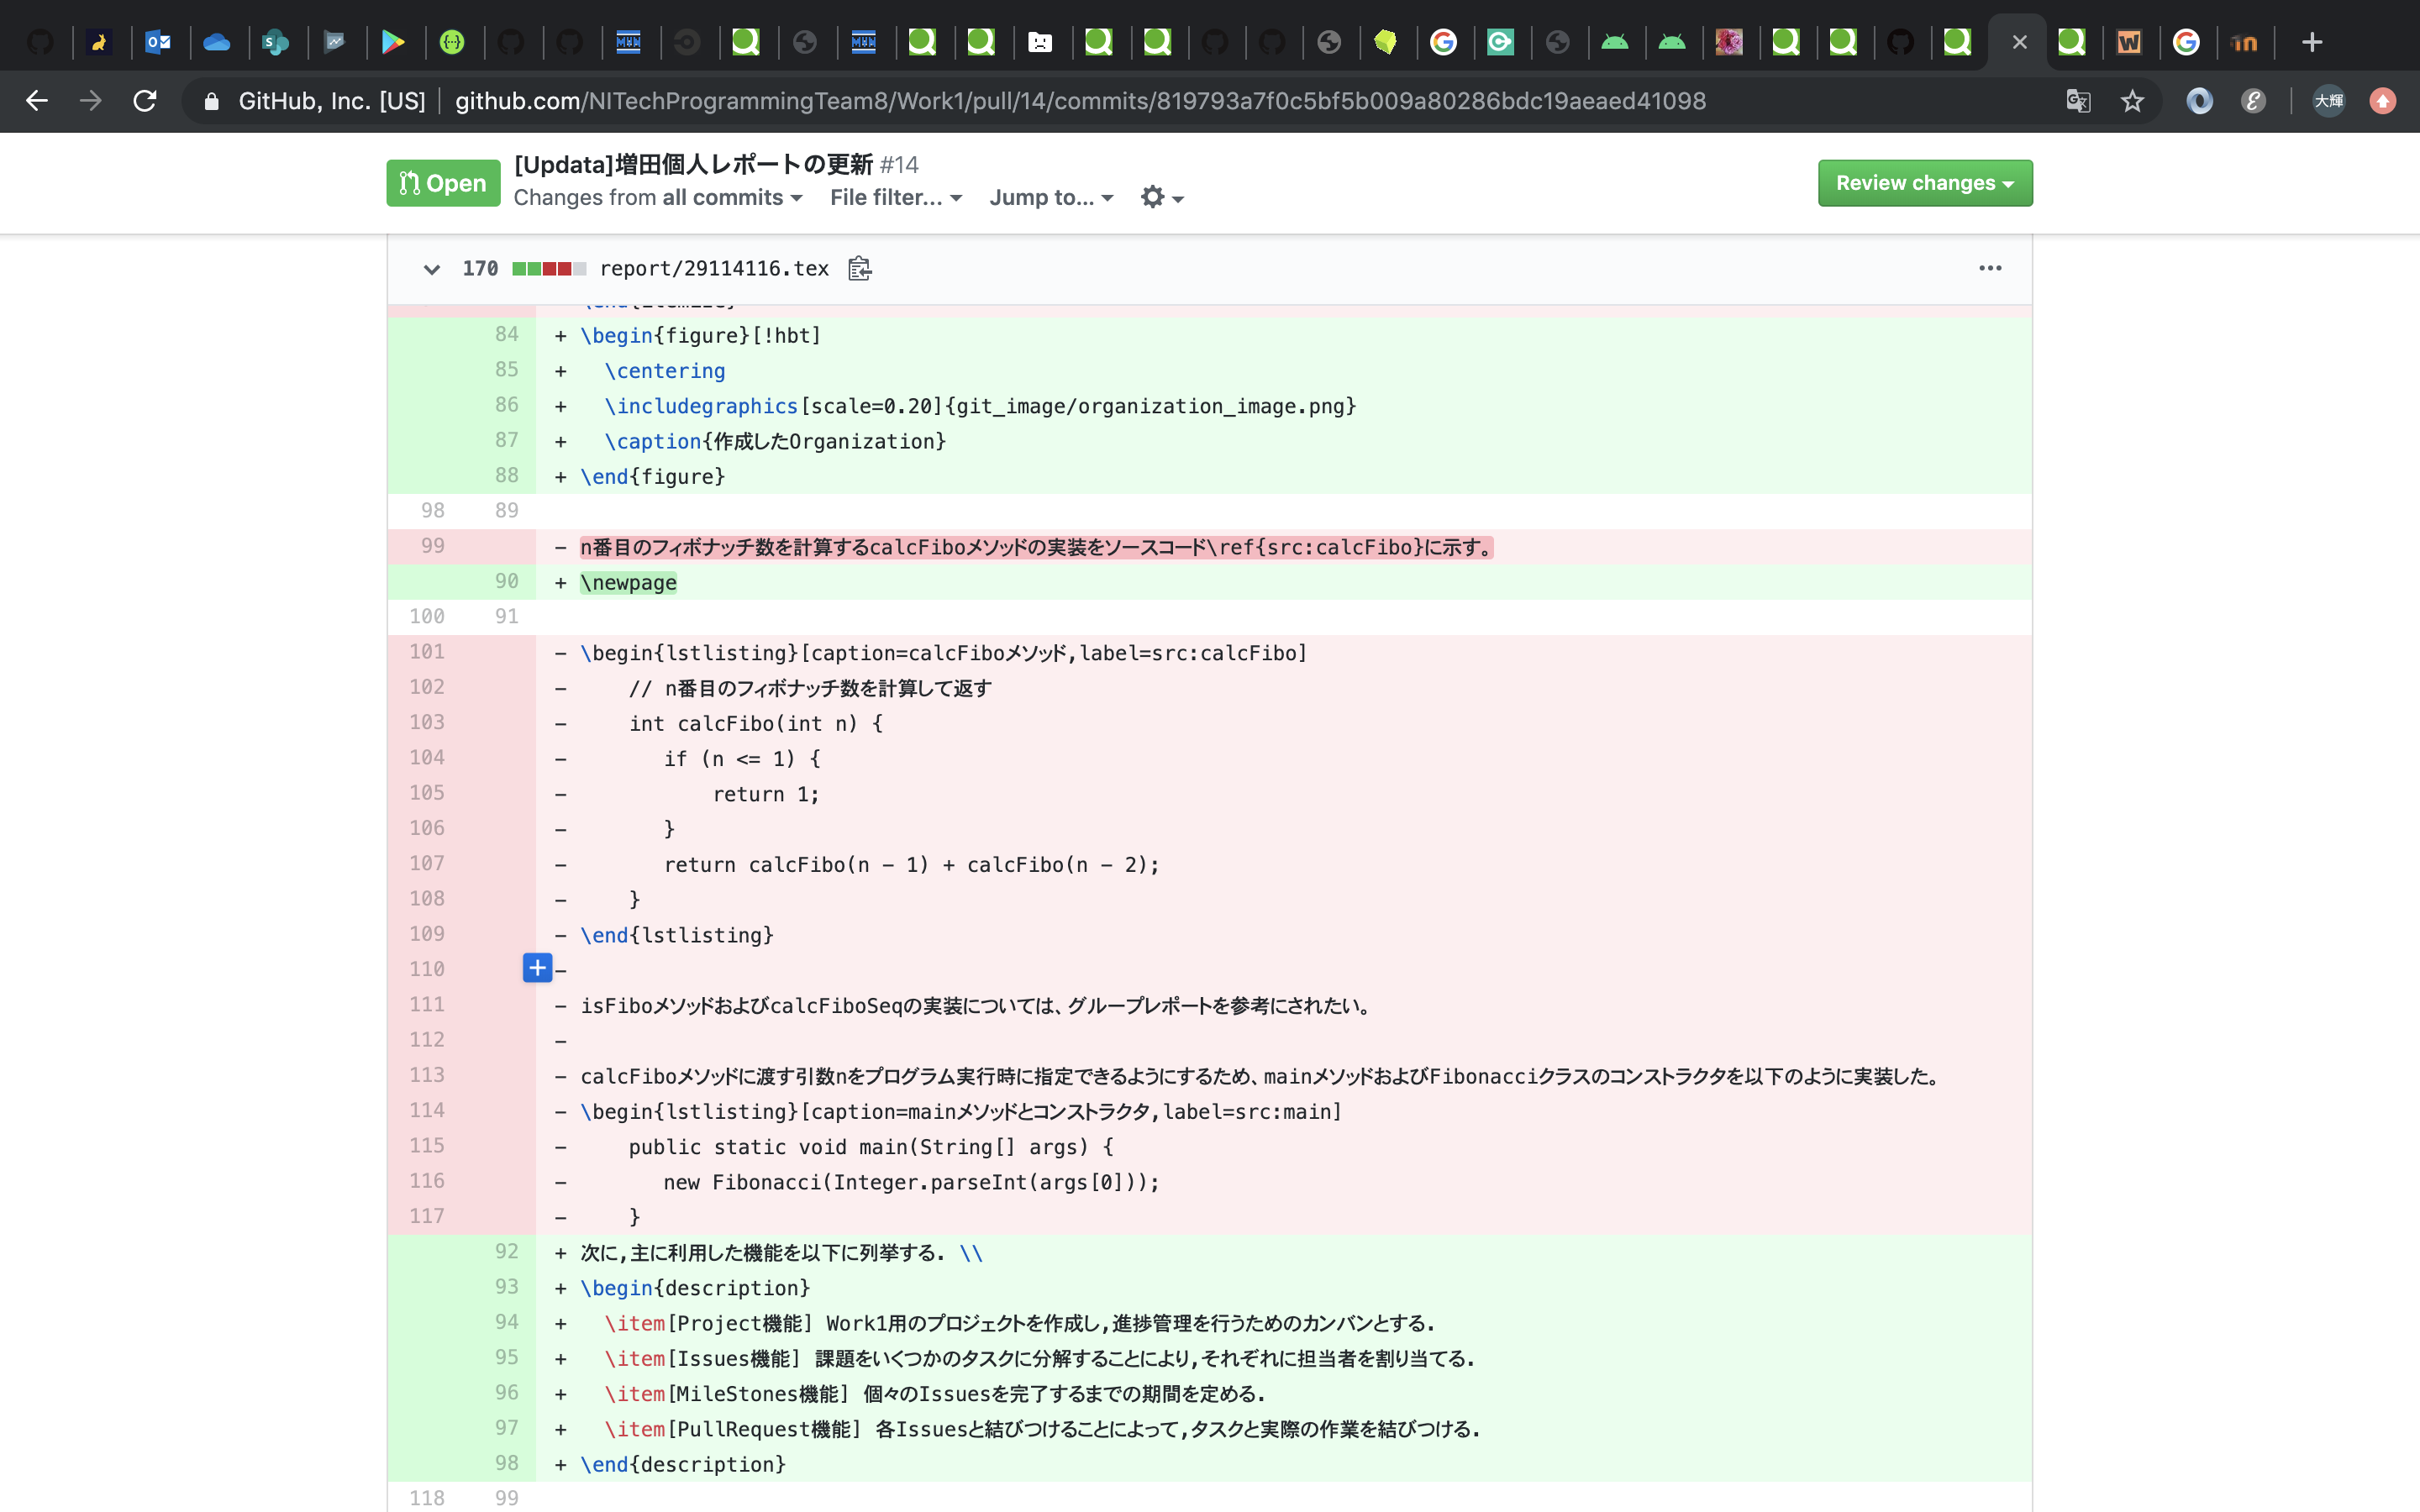
\includegraphics[scale=0.20]{git_image/pull_request_detail_image.png}
  \caption{PRの差分詳細}
\end{figure}

\begin{figure}[!hbt]
  \centering
  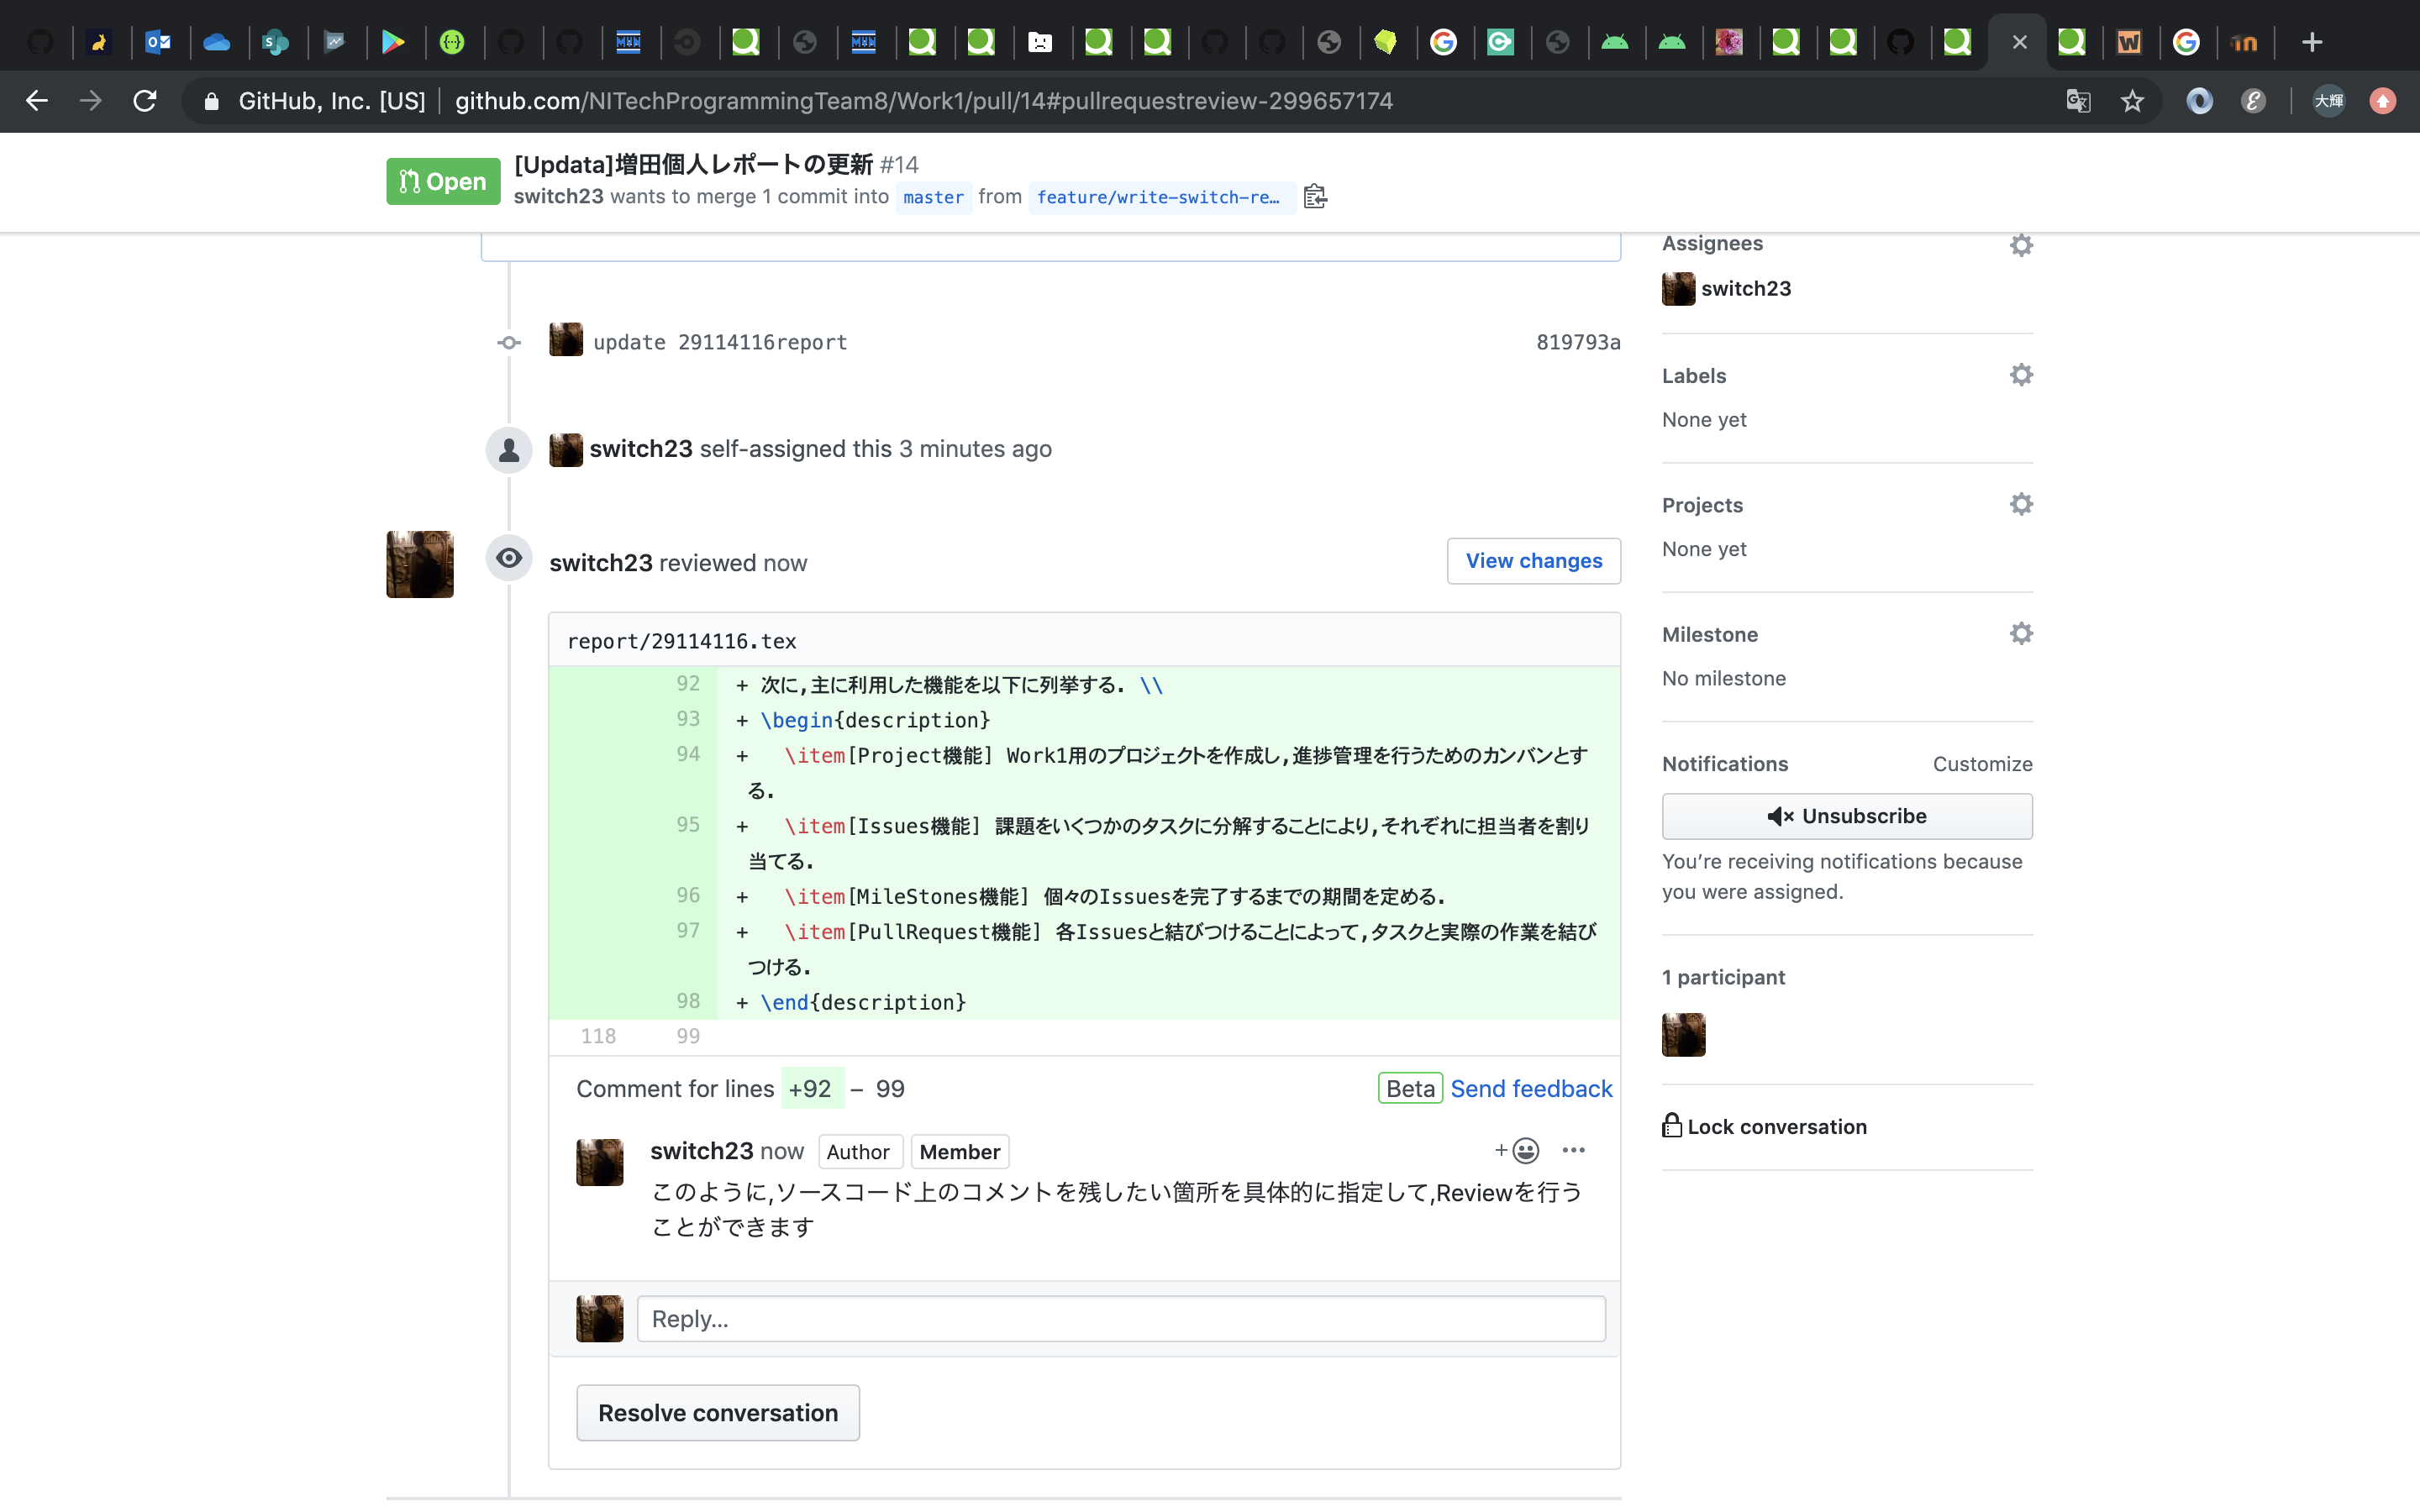
\includegraphics[scale=0.20]{git_image/pull_request_comment_image.png}
  \caption{PRのレビュー機能}
\end{figure}

\newpage


\subsection{チームメンバーへのレクチャー}
チーム開発においては必須と言えるGitHubだが,概念的な理解が必要かつ多機能であるため,学習コストも非常に大きいというデメリットも存在する.
しかし,今後の課題を想定すると,早い段階でGitHubを導入することにより,メンバー全員にGit管理の習慣を定着させることが最善であると判断した.
したがって,学習コストというデメリットを克服する必要があると考えられる.
私は,そのために基本的なGitコマンドの解説や手順を概念的な理解と共に学習できるようにREADME.mdを作成した.
以下に,実際に作成したものを示す.

\begin{figure}[!hbt]
  \centering
  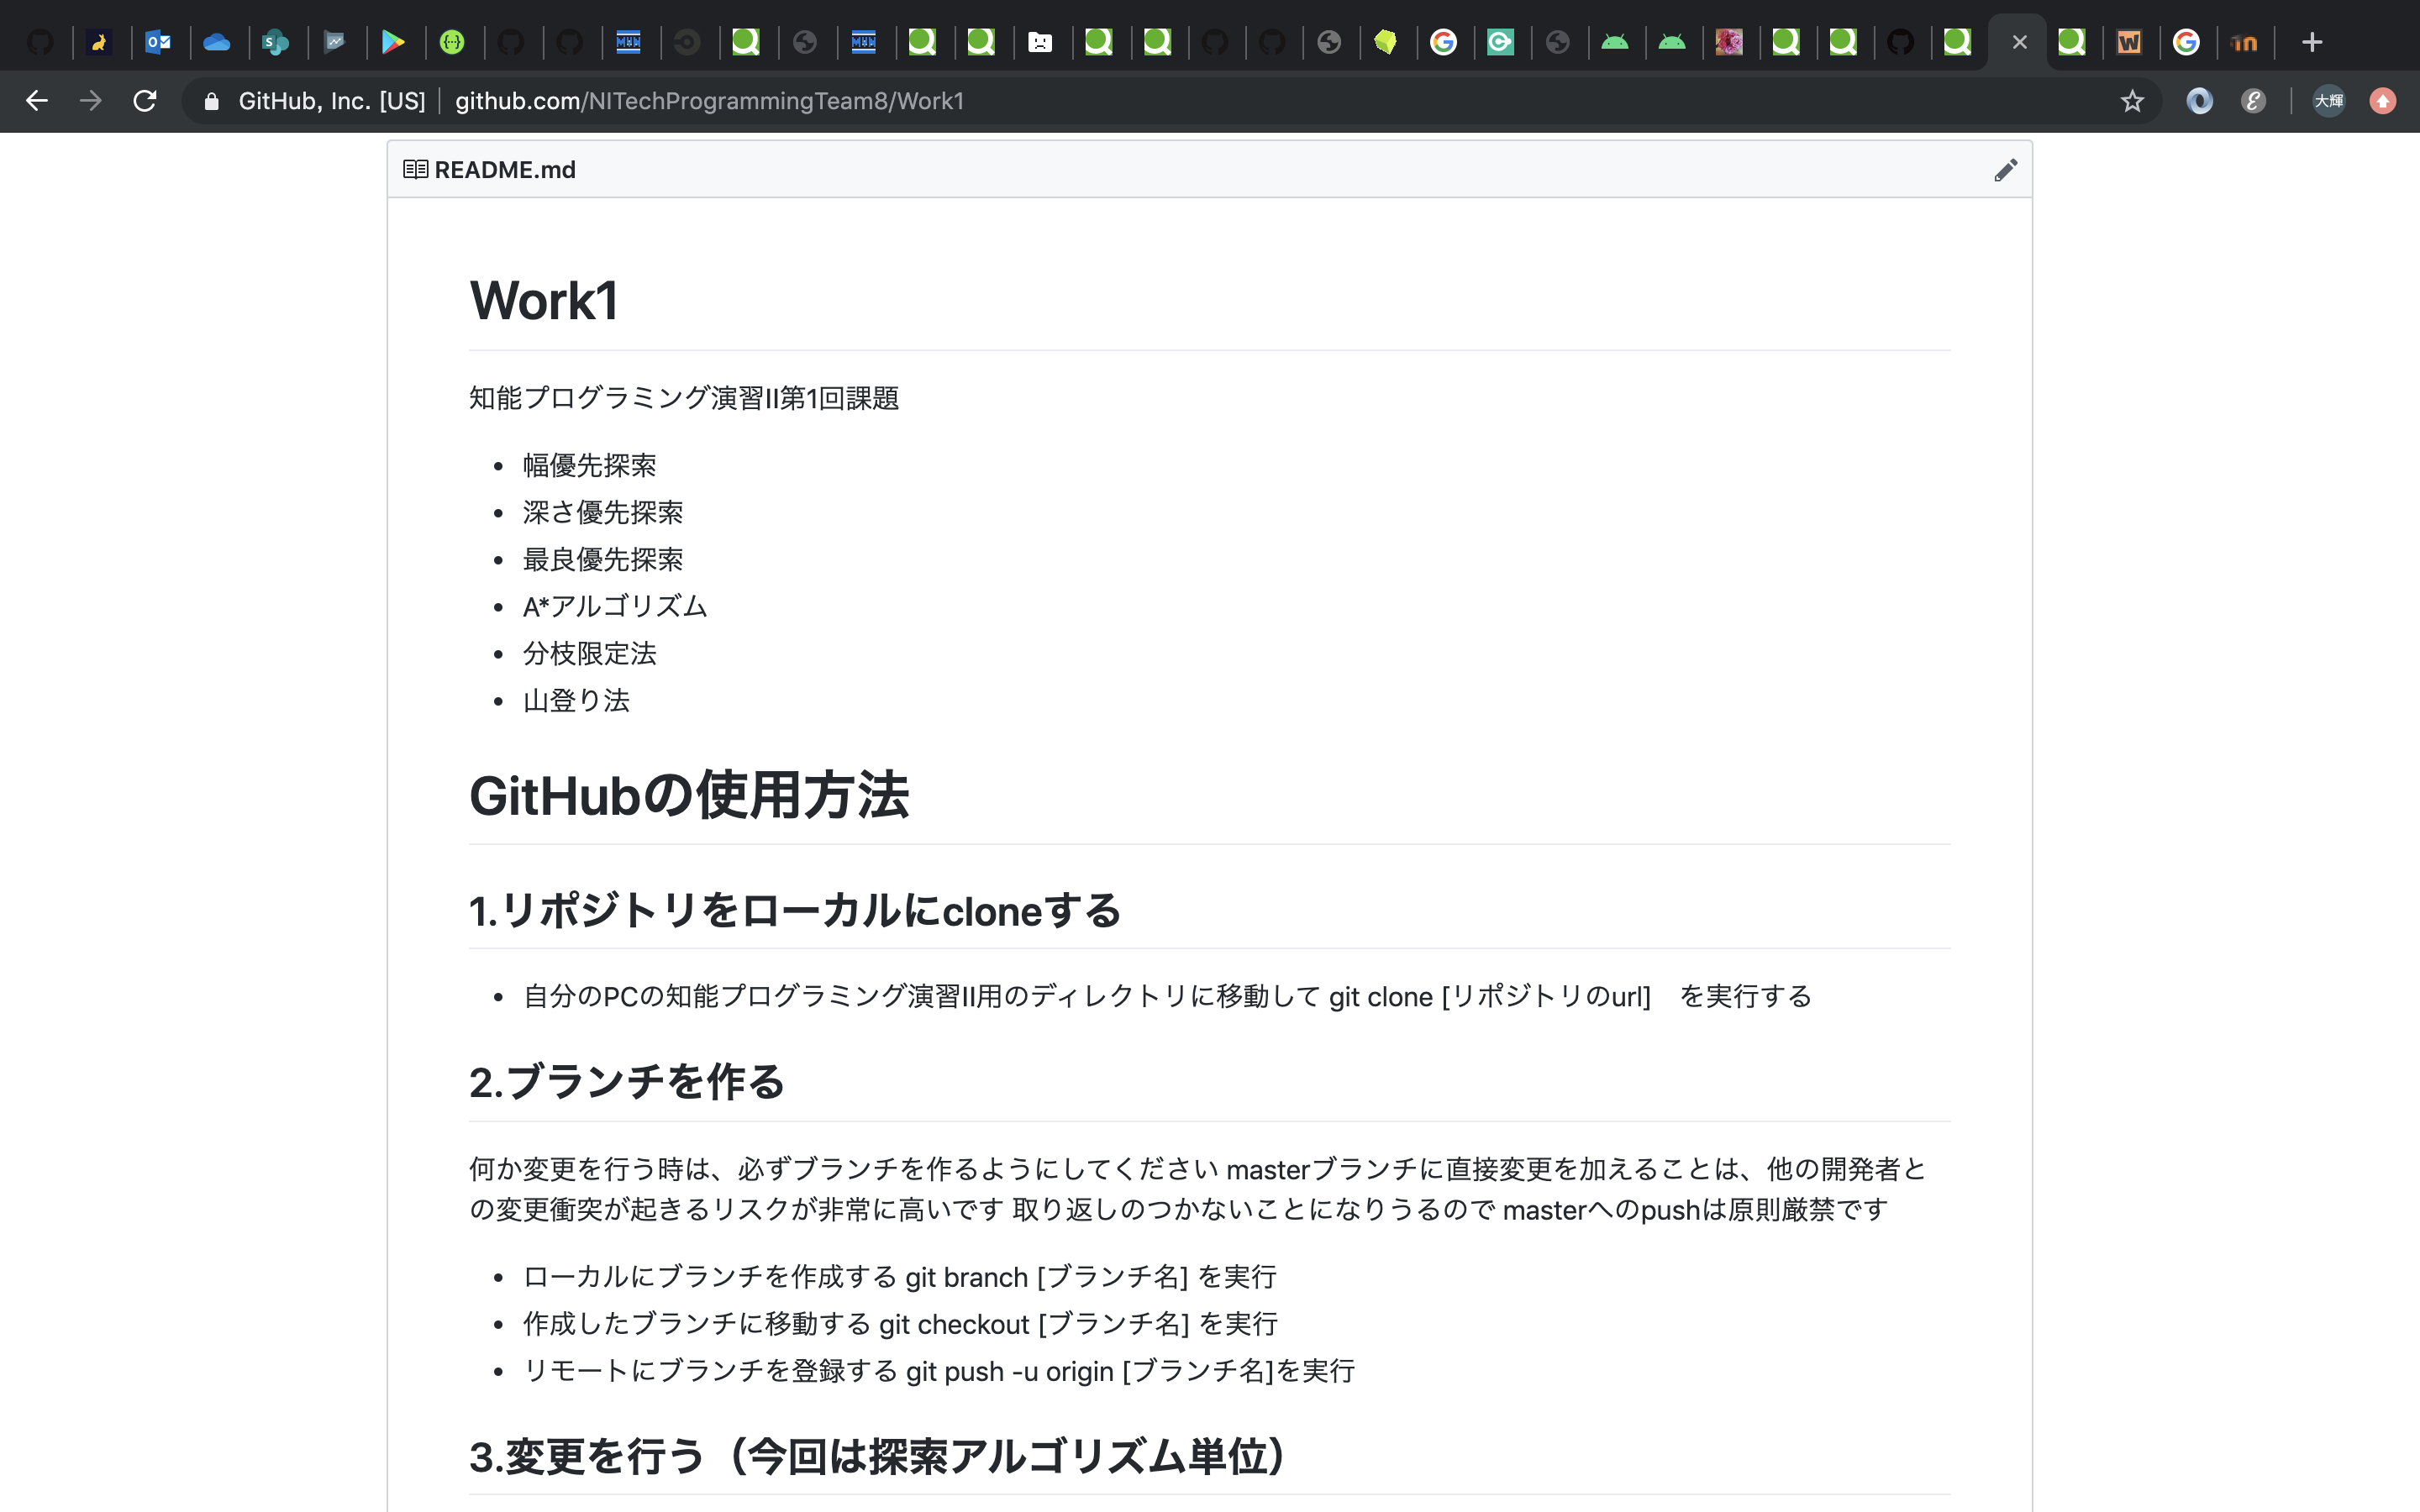
\includegraphics[scale=0.20]{git_image/read_me_1.png}
  \caption{README.mdその1}
\end{figure}

\begin{figure}[!hbt]
  \centering
  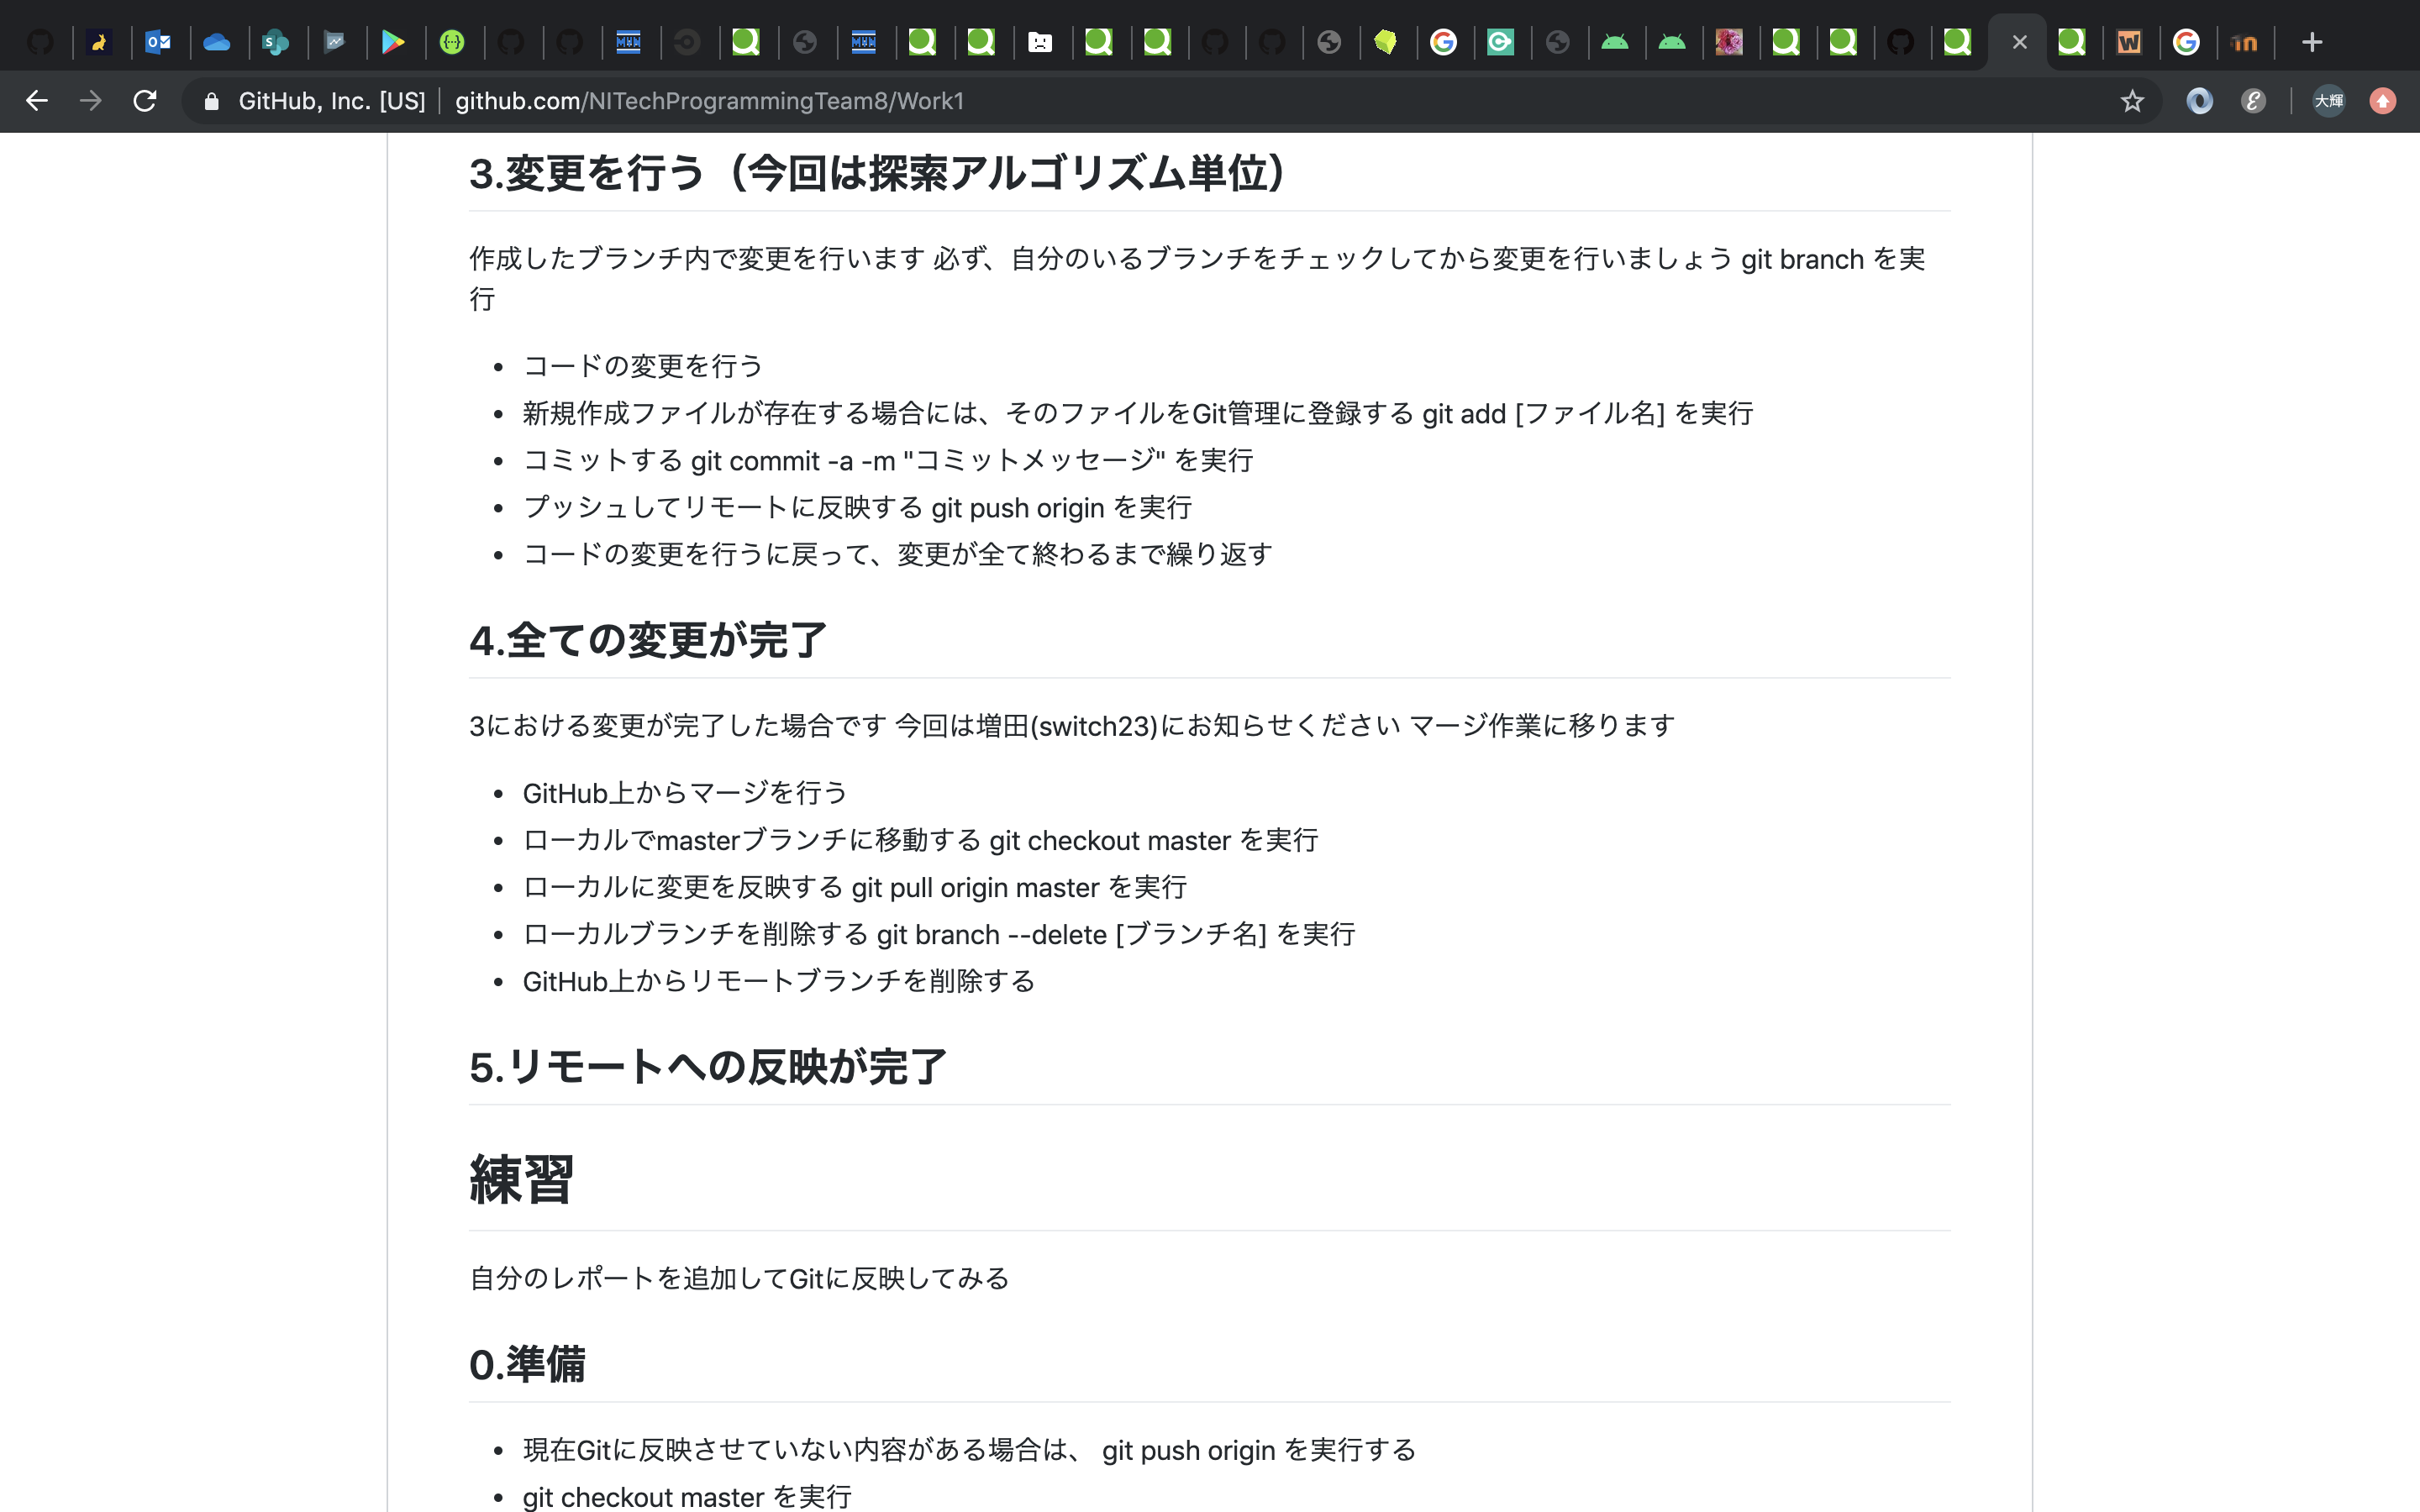
\includegraphics[scale=0.20]{git_image/read_me_2.png}
  \caption{README.mdその2}
\end{figure}

\newpage

\begin{figure}[!hbt]
  \centering
  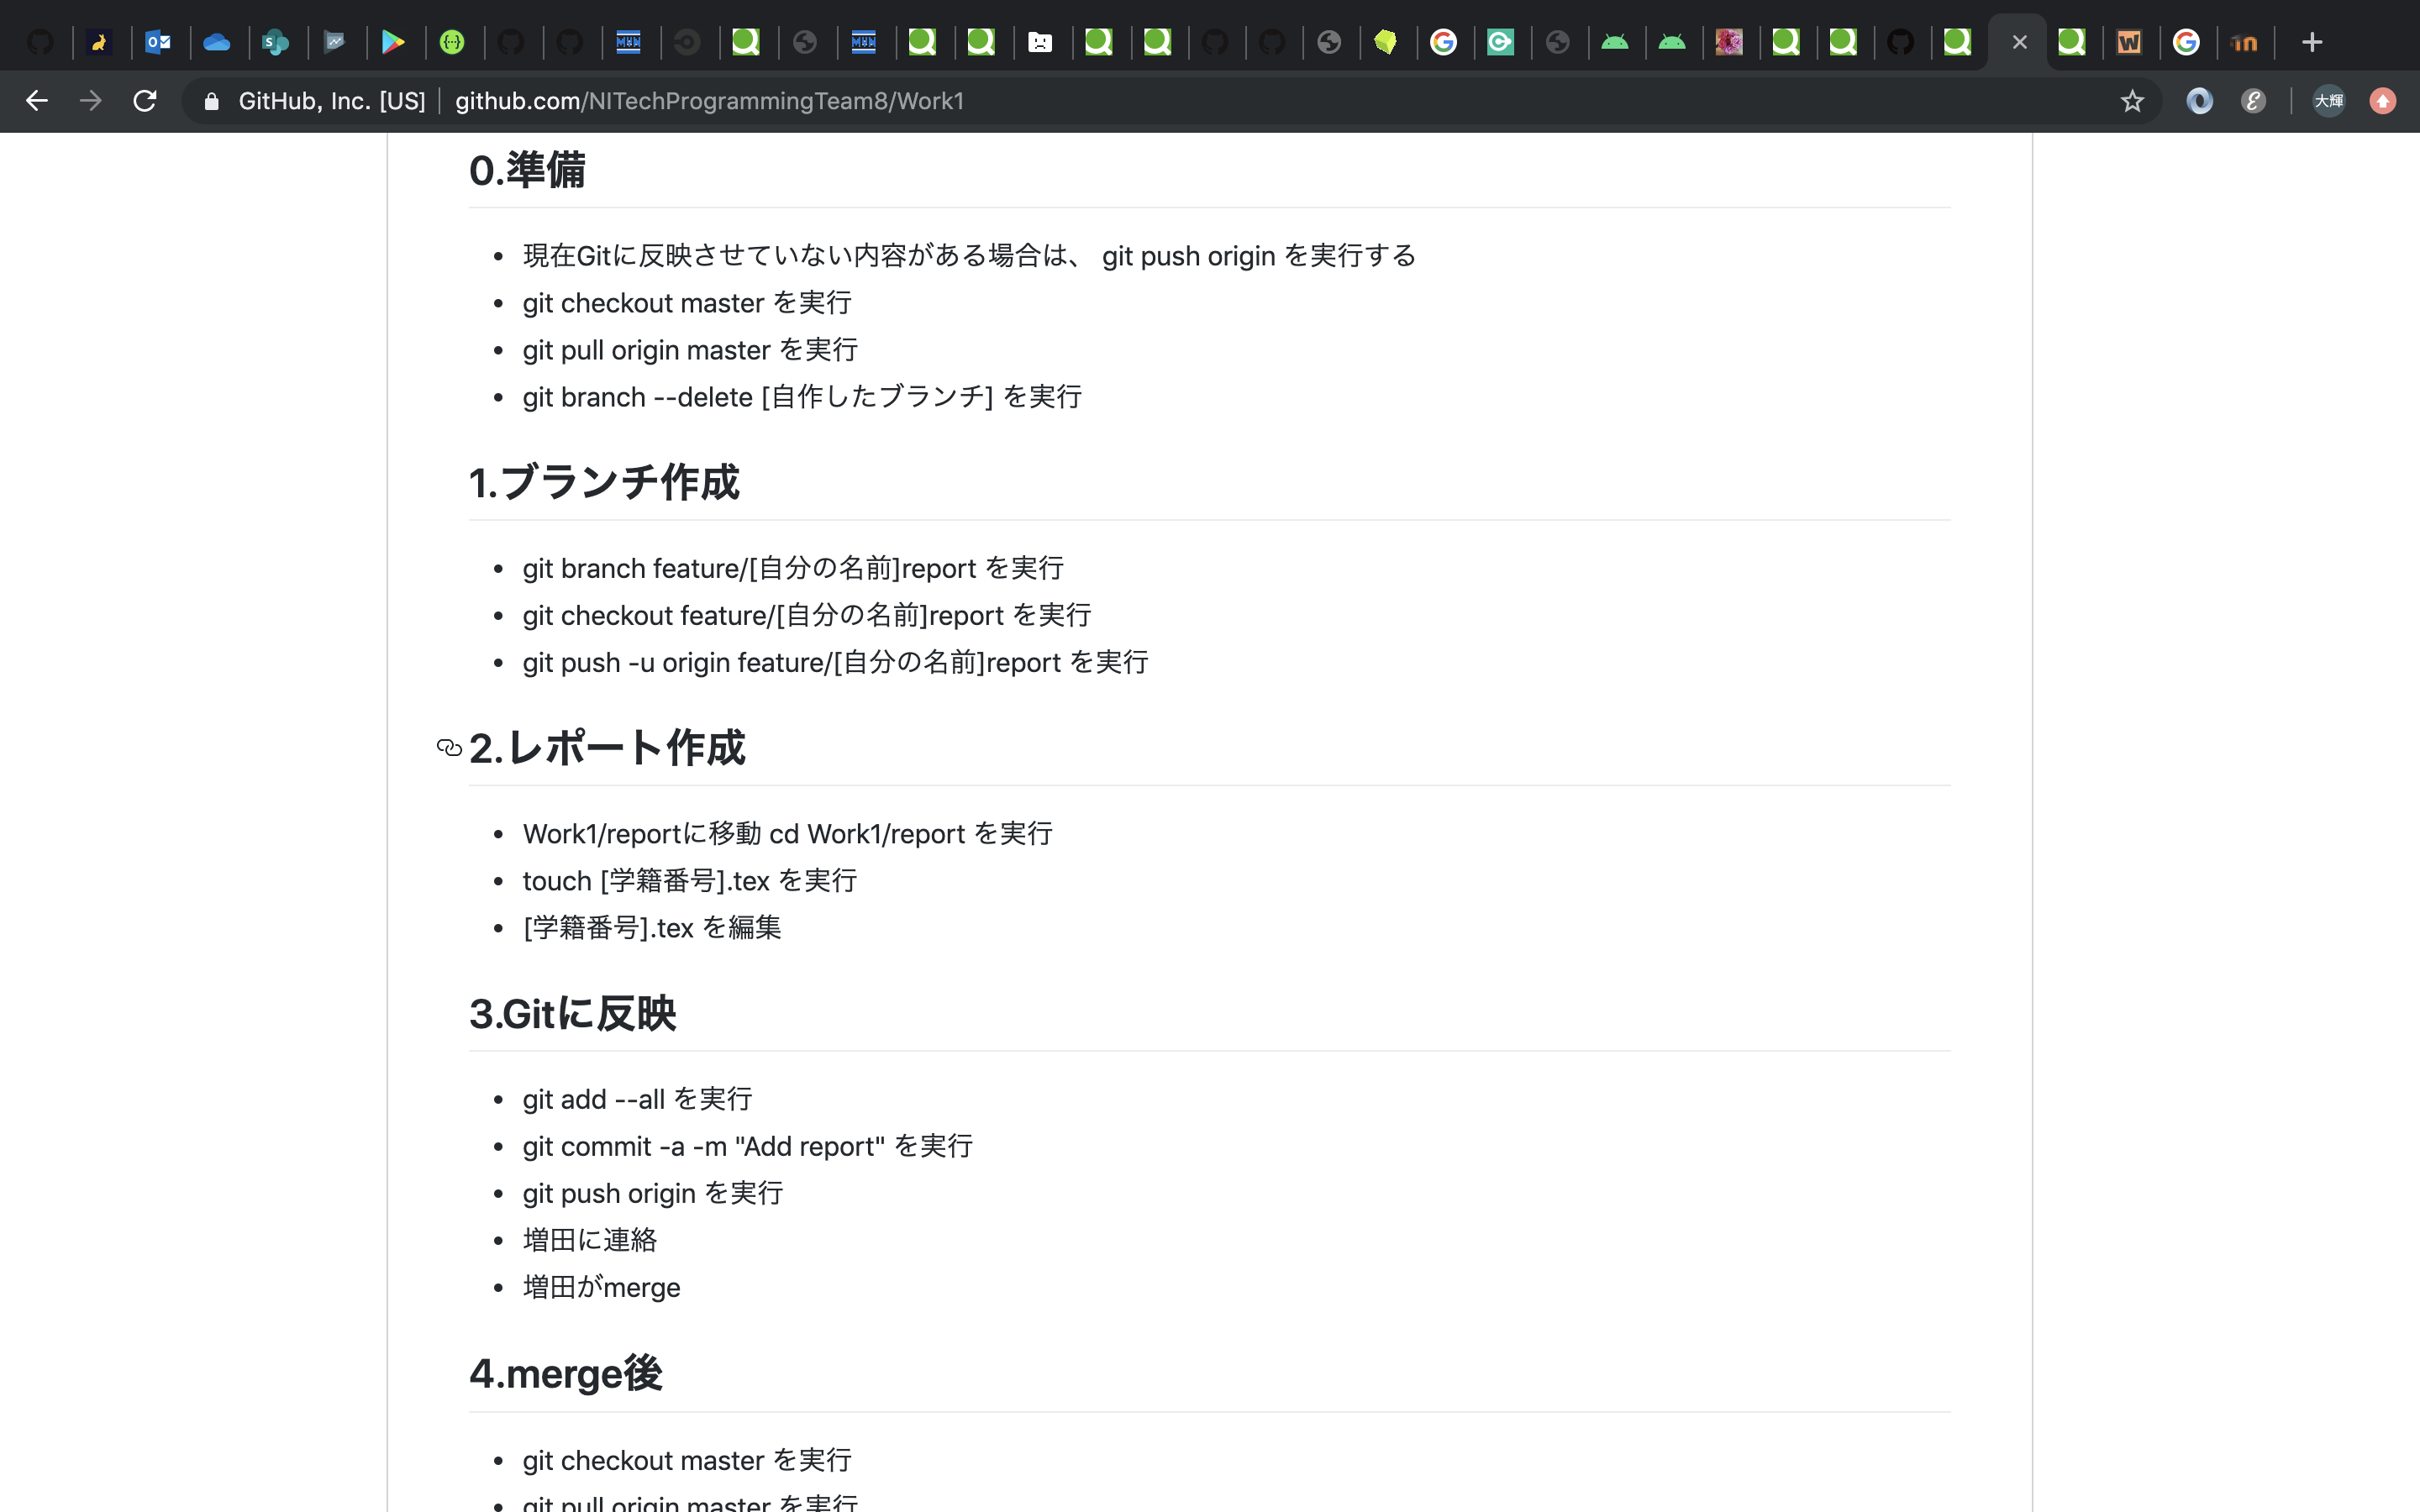
\includegraphics[scale=0.20]{git_image/read_me_3.png}
  \caption{README.mdその3}
\end{figure}

\subsection{Slackの導入}
Slackで専用のワークスペースを作成し,複数のチャンネルを作成した.
具体的には,今回の課題用のチャンネル\#work1と,GitHub運用についてのトピックスを扱うチャンネル\#githubを作成した.

\begin{figure}[!hbt]
  \centering
  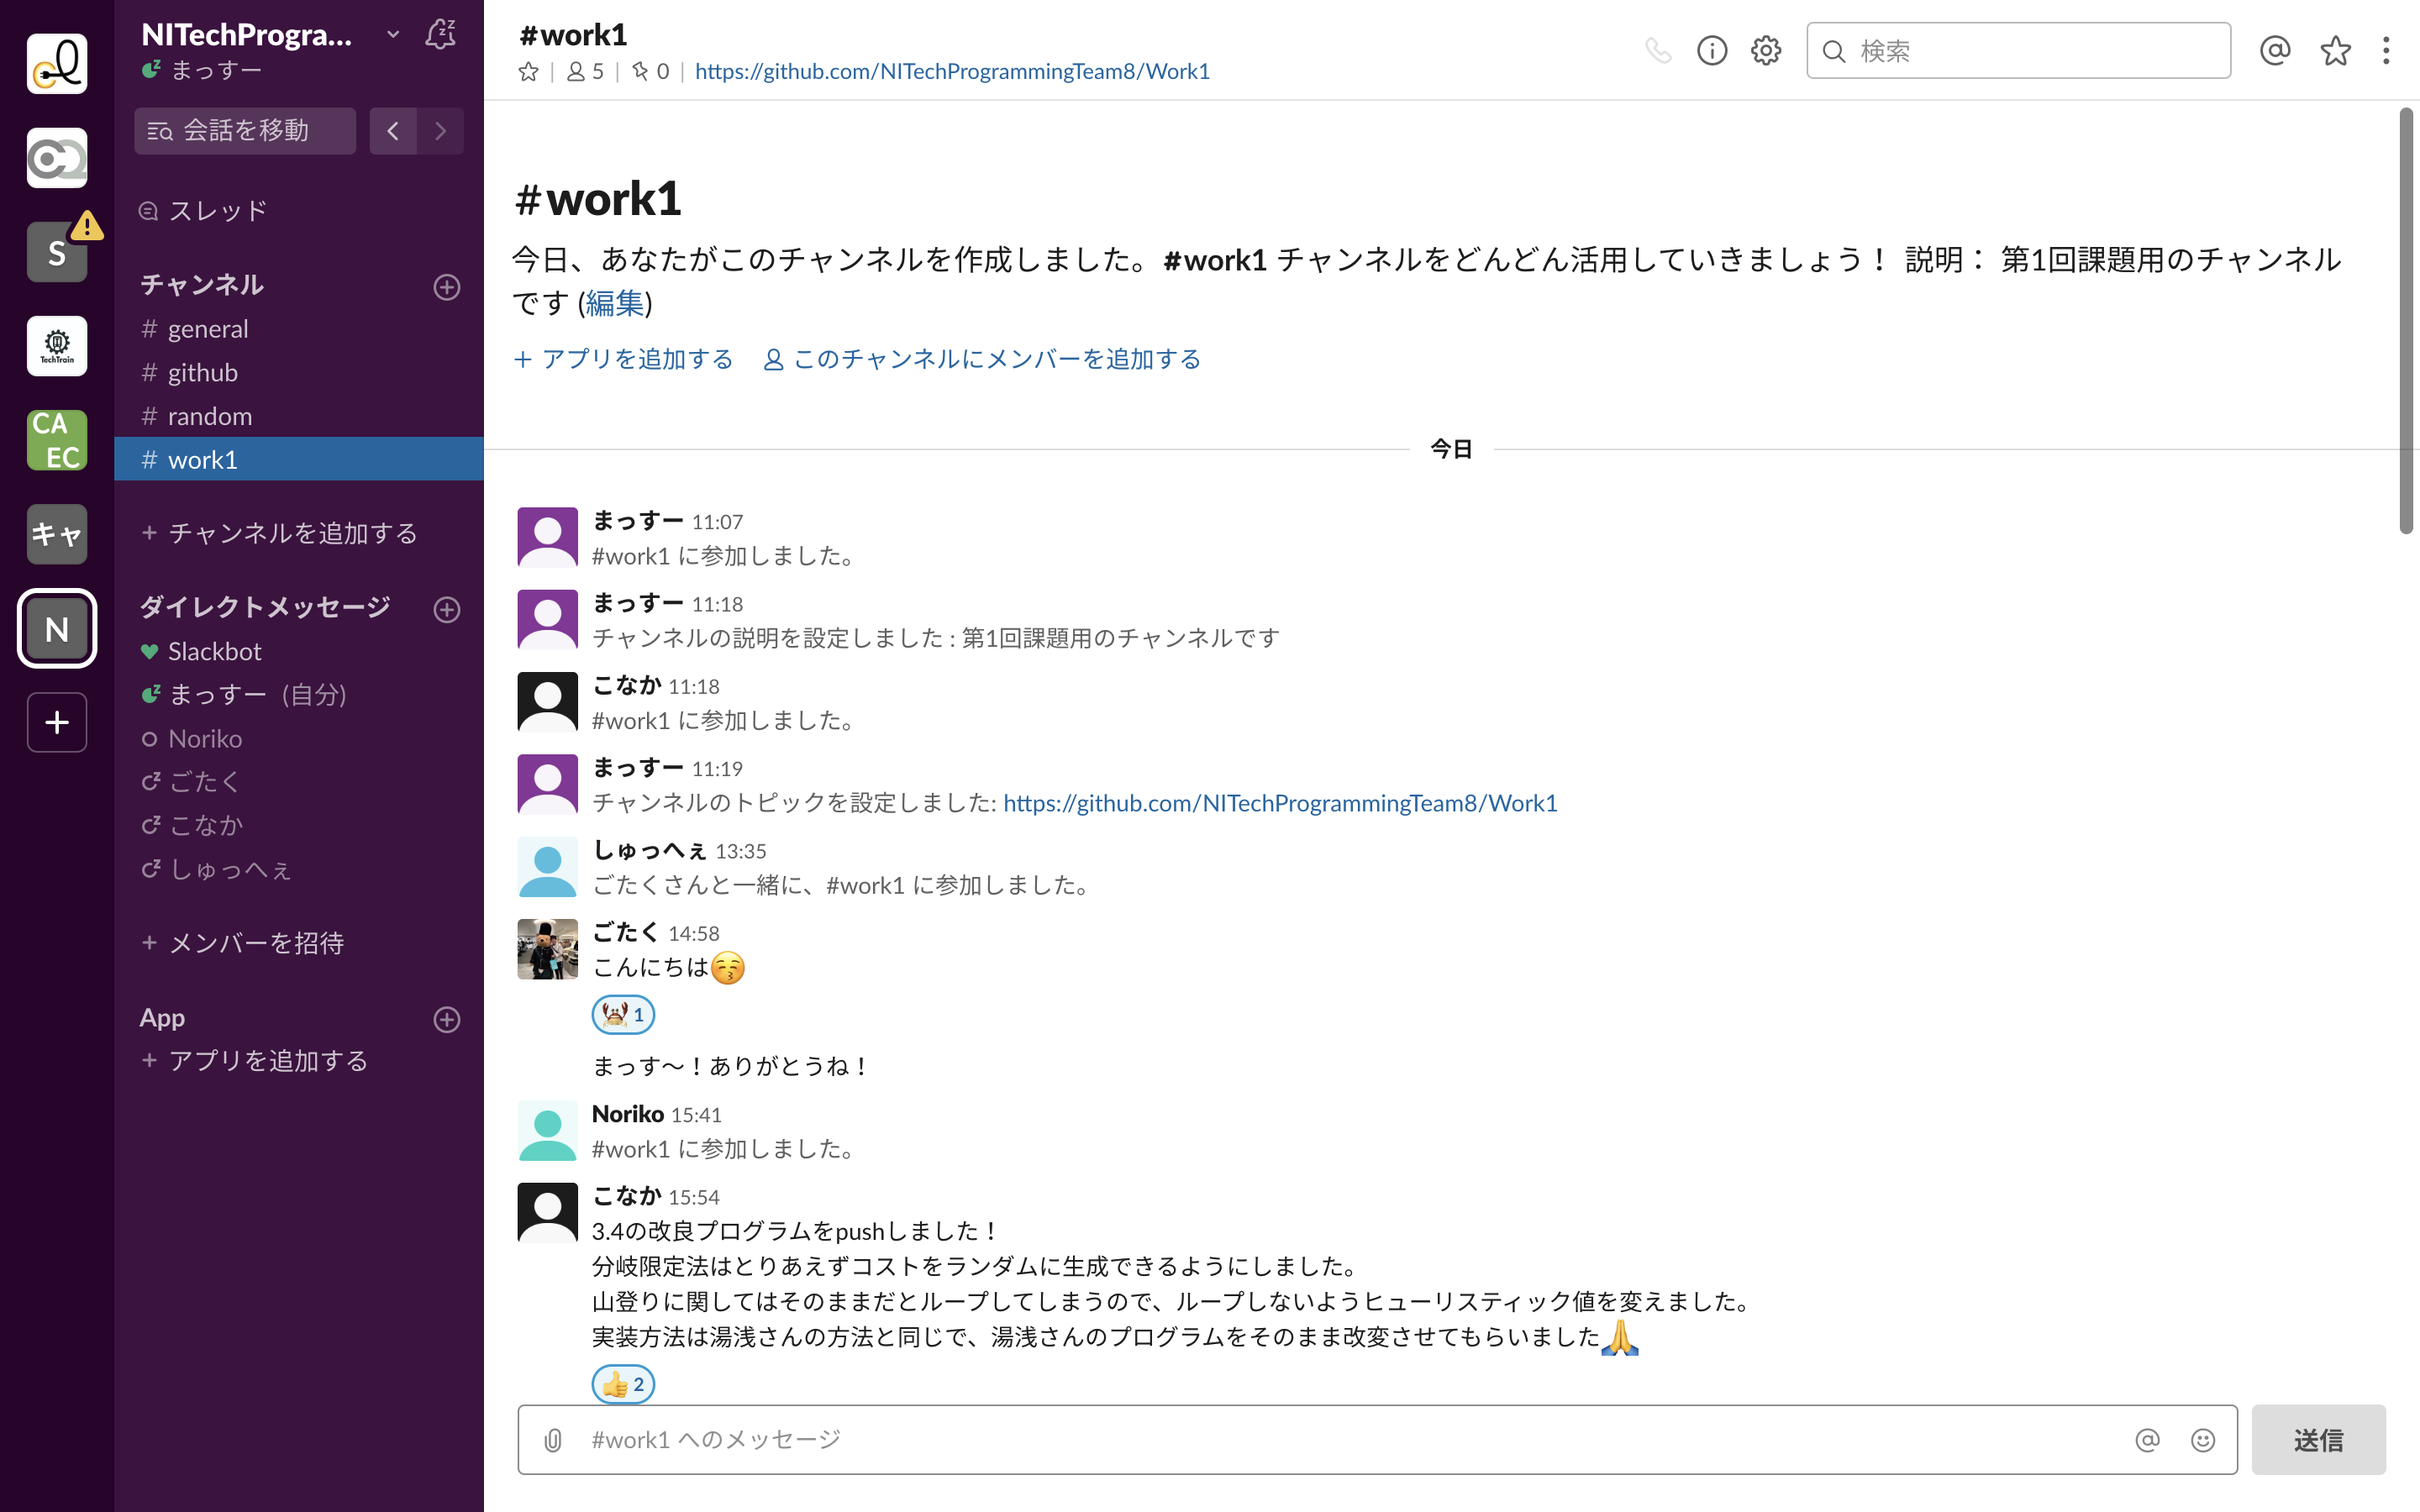
\includegraphics[scale=0.20]{git_image/slack_image.png}
  \caption{README.mdその3}
\end{figure}

% 参考文献
\begin{thebibliography}{99}
\bibitem{notty} 新入社員におくるGitHubでのプロジェクト管理の初歩 --著:hayato ki \\
\url{https://qiita.com/gumimin/items/63dcb36d4730213bd63a} (2019年10月7日アクセス).

\end{thebibliography}

\end{document}